% !TEX TS-program = pdflatex
% !TEX encoding = UTF-8 Unicode
\documentclass[a4paper]{article}
\usepackage[utf8]{inputenc}

%%% PAGE DIMENSIONS ------------------------------------------------------------
\usepackage[bottom=1in]{geometry}
\usepackage[parfill]{parskip}

%%% HEADERS & FOOTERS ----------------------------------------------------------
\usepackage{fancyhdr}
\pagestyle{fancy}

%%% PACKAGES -------------------------------------------------------------------
%\usepackage{morefloats}
\usepackage[hypcap=false,
	font=small,
	labelfont=bf,
	textfont=it]{caption}
\usepackage[pdftex]{graphicx}
\usepackage{tabu}
\usepackage{booktabs}
\usepackage{array}
\usepackage{enumitem}
\usepackage{longtable}
\usepackage{listings}
\usepackage{color}
\usepackage[table]{xcolor}
\usepackage{pdflscape}
\usepackage[percentage]{overpic}
\usepackage{pdfpages}
\usepackage{tikz}
\usetikzlibrary{patterns}
\usepackage[%
	activate={true,nocompatibility},
	final,
	tracking=true,
	kerning=true,
	spacing=true,
	factor=1100,
	stretch=10,
	shrink=10]{microtype}

%% BIBIOGRAPHY -----------------------------------------------------------------
\usepackage{cite}

%%% ToC (table of contents) APPEARANCE -----------------------------------------
% \usepackage[nottoc,notlof,notlot]{tocbibind}
% \renewcommand{\cftsecfont}{\rmfamily\mdseries\upshape}
% \renewcommand{\cftsecpagefont}{\rmfamily\mdseries\upshape}
\setcounter{tocdepth}{2}

%%% PDF LINKS AND STYLE --------------------------------------------------------
% \usepackage[unicode=true,
% 	bookmarks=true,bookmarksnumbered=true,bookmarksopen=true,
% 	bookmarksopenlevel=2, breaklinks=false,pdfborder={0 0 0},backref=false,
% 	colorlinks=false]{hyperref}
\usepackage[bookmarks=true]{hyperref}
\hypersetup{%
	colorlinks=true,       % false: boxed links; true: colored links
	linkcolor=red,          % color of internal links (change box color with linkbordercolor)
	citecolor=green,        % color of links to bibliography
	filecolor=magenta,      % color of file links
	urlcolor=cyan           % color of external links
}

\newcommand\tablewidth{%
	\newgeometry{
	marginparwidth=3.2cm,
	marginparsep=0.8cm,
	left=7.2cm,
	bottom=1in}
	\reversemarginpar
}

\newcommand\marginhead[1]{%
	\vspace{10pt}
	\marginpar{\null #1}
}

\usepackage{enumitem}
\renewcommand{\labelenumii}{\theenumii}
\renewcommand{\theenumii}{\theenumi.\arabic{enumii}.}
\renewcommand{\labelenumiii}{\theenumiii}
\renewcommand{\theenumiii}{\theenumii\arabic{enumiii}.}
\newcommand{\anoun}[1]{\textcolor{red}{\textbf{#1}}}
\newcommand{\averb}[1]{\textcolor{blue}{\textbf{#1}}}

%*******************************************************************************
%******************************** END HEADER ***********************************
%*******************************************************************************

\begin{document}

%!TEX root = mainfile.tex
\begin{titlepage}
	\begin{center}
	\vspace*{\fill}

	\centering
	
\includegraphics[scale=1.2]{Logo.pdf}
	\vfill

	\hrule
	{\LARGE\bf Software Engineering \\
		--- \\
		Online Travel \& Hotel Booking System (Travpedia)\\[0.4cm]}
	\hrule

	\vfill
	% \large
	% School of Computer Science\\
	% University of Birmingham

	\vfill
		Rebecca Devney,\\
		Julie Sewards,\\
		Andrew Walker,\\
		Josh Wainwright
	\vfill
	Travel and All That

	\vfill
	\vfill
	\textit{Date:} April 2014
	\vfill
	\vfill

	\end{center}
\end{titlepage}

%\thispagestyle{empty}
%\vspace*{\fill}
%\noindent
%\begin{tabular}{ll}
%\end{tabular}

%\cleardoublepage
%\cleardoublepage

\mbox{}
\thispagestyle{empty}

\tableofcontents
\clearpage
\setcounter{page}{1}

\section{Specification}

Travpedia is an online travel and accommodation booking system. Travel and
accommodation companies are able to subscribe to Travpedia for a monthly
subscription cost of £200 plus an initial £50 joining fee. This subscription
allows the company to offer their products on the Travpedia website where they
can be purchased by visiting users. Products that are advertised on the
Travpedia website include accommodation, package holidays and travel by air,
rail and sea. One or more products may be combined into a single booking.

Visitors to the website, after registering an account, are able to search for
all available products offered by these subscribed companies. They are able to
search with a number of criteria including type of product, location, date and
price. Users can then view these search results and book and pay for products
through the website. Users may also rate and review accommodation and package
holidays that they have purchased. A product gains a review score based on
these ratings. This review rating system provides further search criteria
whereby a user can filter search results by review score.

Payments made by both subscribing companies and users are handled online by a
third party consortium. Subscribers must pay by debit or credit card while
users have the additional option of paying with gift vouchers offered by
Travpedia.

Users are able to view bookings they have made and, where possible, cancel
these bookings and receive a refund via the third party consortium.

Travpedia disseminates advertisements and promotional offers to users based on
previous patterns of use and previous purchases. These personalised offering
are sent to mobile phones through SMS and email accounts. Users may opt out of
receiving SMS and email alerts.

Travpedia also has a number of critical compliance and security requirements.
Travpedia stores users' personal information and payment details that should
not be disclosed to other parties or kept for any longer than necessary. If
this data is maliciously accessed, disclosed, leaked or manipulated it could
breach confidentiality and data protection. Furthermore, any transaction
information sent to the third party consortium used for payment must be kept
secure. This is done with encryption using 128-bit SSL certificates.

During peak time, Travpedia receives up to one million simultaneous users and
is designed to handle this number of users. The design is also scalable to
accommodate its growing number of users and subscribers. This system is used
by users 24 hours a days and must be always available. All data that Travpedia
stores must also be kept safe from system failures. For this reason, user
account details, itinerary and transaction data and subscribers' data are
stored and backed up on three database servers in three distinct locations. Two
of these locations are in the UK and the other is in the USA. This allows
Travpedia to minimise downtime after unforeseen system failures.

\subsection{Scope}

The scope of our design is limited primarily to subsystems devoted to user's
interactions with the Travpedia website. In particular, we will consider the
following:

\begin{itemize}
	\item Travpedia account registration.
	\item Searching for products.
	\item Making new bookings.
	\item Viewing and cancelling previous bookings.
\end{itemize}

\subsection{Assumptions}

We have made a number of assumptions regarding the external systems and
remaining internal subsystems described in the whole system specification. We
assume that these other subsystems have their own interface with which we can
communicate when necessary.

\begin{description}
	\item [{Subscribers}] All aspects of company subscriptions to Travpedia
		are handled by the Subscriber Subsystem.
	\item [{Consortium}] The third party consortium will deal with all aspects
		of forwarding user payments to Travpedia's subscribers. We will be
		responsible for sending user payments to this consortium who will then
		respond accordingly about the success of the transaction.
	\item [{Global Distribution System}] A system used by travel and
		accommodation booking agents which acts as an intermediary, providing
		information and an operational interface. Our system will use this
		agency to handle all external booking procedures.
	\item [{User~Database}] There is a database for user profile and account
		data. We can make requests to this database to retrieve and update
		this data.
	\item [{Product~Database}] There is a database for all travel and
		accommodation product data. We can make requests to this database to
		retrieve and update this data.
	\item [{Backup}] In the case of both databases, we assume that, as part of
		the functionality of the databases, backups are made regularly ensuring
		this data is stored across the three distinct database locations.
		Finally, this subsystem also ensures that data is not held longer than
		necessary in order to comply with the Data Protection Act.
	\item [{Recommendations}] Users can receive additional product
		recommendations by email and/or phone notifications. Our system will
		provide the user with the option to receive, or opt out of these, but
		the Recommendation Subsystem deals with the selection and dissemination
		of this information.
\end{description}

\clearpage
\section{Requirements}

\subsection{Functional Requirements}

\begin{enumerate}
	\item Registration

		\begin{enumerate}
			\item The system shall allow the user to register for a new account.

				\begin{enumerate}
					\item The system shall require the user to provide a name and valid email
						address
					\item The system shall require the user to choose and enter a password for
						his/her account
					\item The system shall contact the user by email to confirm that registration
						is complete
				\end{enumerate}
			\item Logging in

				\begin{enumerate}
					\item The system shall require the user to log in using their registered
						email address and password in order to use the facilities offered
						by Travpedia via the website
				\end{enumerate}
		\end{enumerate}
	\item User Account

		\begin{enumerate}
			\item The system shall allow the user to view his/her account details
			\item The system shall allow the user to amend his/her account details
			\item The system shall allow the user to save payment information in his/her
				account
			\item The system shall allow the user to save mailing preference information
				in his/her account
		\end{enumerate}
	\item Search

		\begin{enumerate}
			\item The system shall allow a user to search for products using a combination
				of one or more criteria

				\begin{enumerate}
					\item The system shall allow the user to search by type of product
					\item The system shall allow the user to search by specifying a target price
						range
					\item The system shall allow the user to search for accommodation and/or
						package holidays by location
					\item The system shall allow the user to search for accommodation and/or
						package holidays by specifying a start date and an end date
					\item The system shall allow the user to search for travel by point of departure
						and/or destination
					\item The system shall allow the user to search for travel by specifying
						a start date and, optionally, a return date
					\item The system shall allow the user to specify the number of rooms required
					\item The system shall allow the user to specify the number of seats required
				\end{enumerate}
			\item The system shall enable the user to filter search results

				\begin{enumerate}
					\item The system shall enable the user to filter results by price range
					\item The system shall enable the user to filter accommodation results by
						star rating
				\end{enumerate}
			\item The system shall enable the user to sort search results

				\begin{enumerate}
					\item The system shall enable the user to sort results by price
					\item The system shall enable the user to sort results by review score
					\item The system shall enable the user to sort accommodation results by
						star rating
					\item The system shall enable the user to sort travel results by departure
						time
				\end{enumerate}
		\end{enumerate}
	\item Make a new booking

		\begin{enumerate}
			\item The system shall allow the user to make a new accommodation booking
			\item The system shall allow the user to make a new travel booking
			\item The system shall allow the user to make a new package holiday booking
			\item The system shall allow the user combine one or more products into
				a single booking
		\end{enumerate}
	\item View or cancel an existing booking

		\begin{enumerate}
			\item The system shall allow the user to view an existing booking
			\item The system shall allow the user to cancel a booking
		\end{enumerate}
	\item Make a payment

		\begin{enumerate}
			\item The system shall allow the user to make a payment by either or both
				of the following

				\begin{enumerate}
					\item The system shall allow the user to pay by credit/debit card
					\item The system shall allow the user to pay by Travpedia voucher
				\end{enumerate}
			\item The system shall send the user an email to their registered email
				address confirming details of the completed payment.
		\end{enumerate}
\end{enumerate}

\subsection{Non-Functional Requirements}

\subsubsection{Product Requirements}
\begin{enumerate}
	\item Efficiency

		\begin{enumerate}
			\item The system shall respond to a search request in under 10 seconds
			\item The system shall respond to a user login request within 3 seconds
			\item The system shall send all confirmation emails withing 2 minutes.
			\item The system shall be capable of handling 1 million simultaneous users
				during peak time.
		\end{enumerate}
	\item Dependability

		\begin{enumerate}
			\item The system shall be available 24/7 for 99\% of the time. (Availability)
			\item The system shall require users to confirm all booking and payment
				transactions before executing to mitigate against user error (Error-tolerance)
			\item The system will operate a mirror server - the principal and mirror
				servers will be located at geographically separate locations in the
				UK.
			\item The system will provide a further database server in the USA in order
				to facilitate disaster recovery.
		\end{enumerate}
	\item Usability

		\begin{enumerate}
			\item The system shall be easy to use (as evidenced by 80\% positive feedback
				from 'usability' questions on user satisfaction questionnaires).
			\item The system shall provide the user with context specific help.
			\item The system shall provide the user with information on the progress
				of all searches taking more than 3 seconds.
		\end{enumerate}
	\item Security

		\begin{enumerate}
			\item The system should block user access after 5 consecutive failed login
				attempts
			\item The system shall secure and encrypt all financial transactions passed
				to the third party consortium using 128-bit SSL certificates
			\item The system shall secure and encrypt all user data passed to the Global
				Distribution System (GDS) using 128-bit SSL certificates
		\end{enumerate}
\end{enumerate}

\subsubsection{Organisational Requirements}
\begin{enumerate}
	\item Development

		\begin{enumerate}
			\item The system shall operate on all major web browsers e.g. Internet Explorer,
				Firefox, Chrome, Safari
			\item The system shall operate on both desktop and mobile platforms
		\end{enumerate}
	\item Standards

		\begin{enumerate}
			\item The system shall conform with all requirements laid down in the company's
				ISO 9001:2008 Quality Management Procedures
		\end{enumerate}
\end{enumerate}

\subsubsection{External Requirements}
\begin{enumerate}
	\item Interoperability

		\begin{enumerate}
			\item The system shall integrate with the GDS in order to ensure correct
				processing of user bookings
			\item The system shall correctly integrate with the third party consortium
				that handles payments
		\end{enumerate}
	\item Legislative \& Ethical

		\begin{enumerate}
			\item The system shall comply with the Payment Card Industry Data Security
				Standards (PCI DSS)
			\item The system shall comply with all requirements of the UK Data Protection
				Act 2003.
			\item The system shall comply with level AA of the Web Content Accessibility
				Guidelines.
		\end{enumerate}
\end{enumerate}

\clearpage

\section{Use Case Diagram}

The use case diagram below represents a user's interaction with the Travpedia
system and the ways in which these actions are handled by the system and
external and third party systems. Each use case is a simple view of what would
be a more complex series of events to realise it.

\begin{figure}[h!]
	\centering
	\makebox[\textwidth][c]{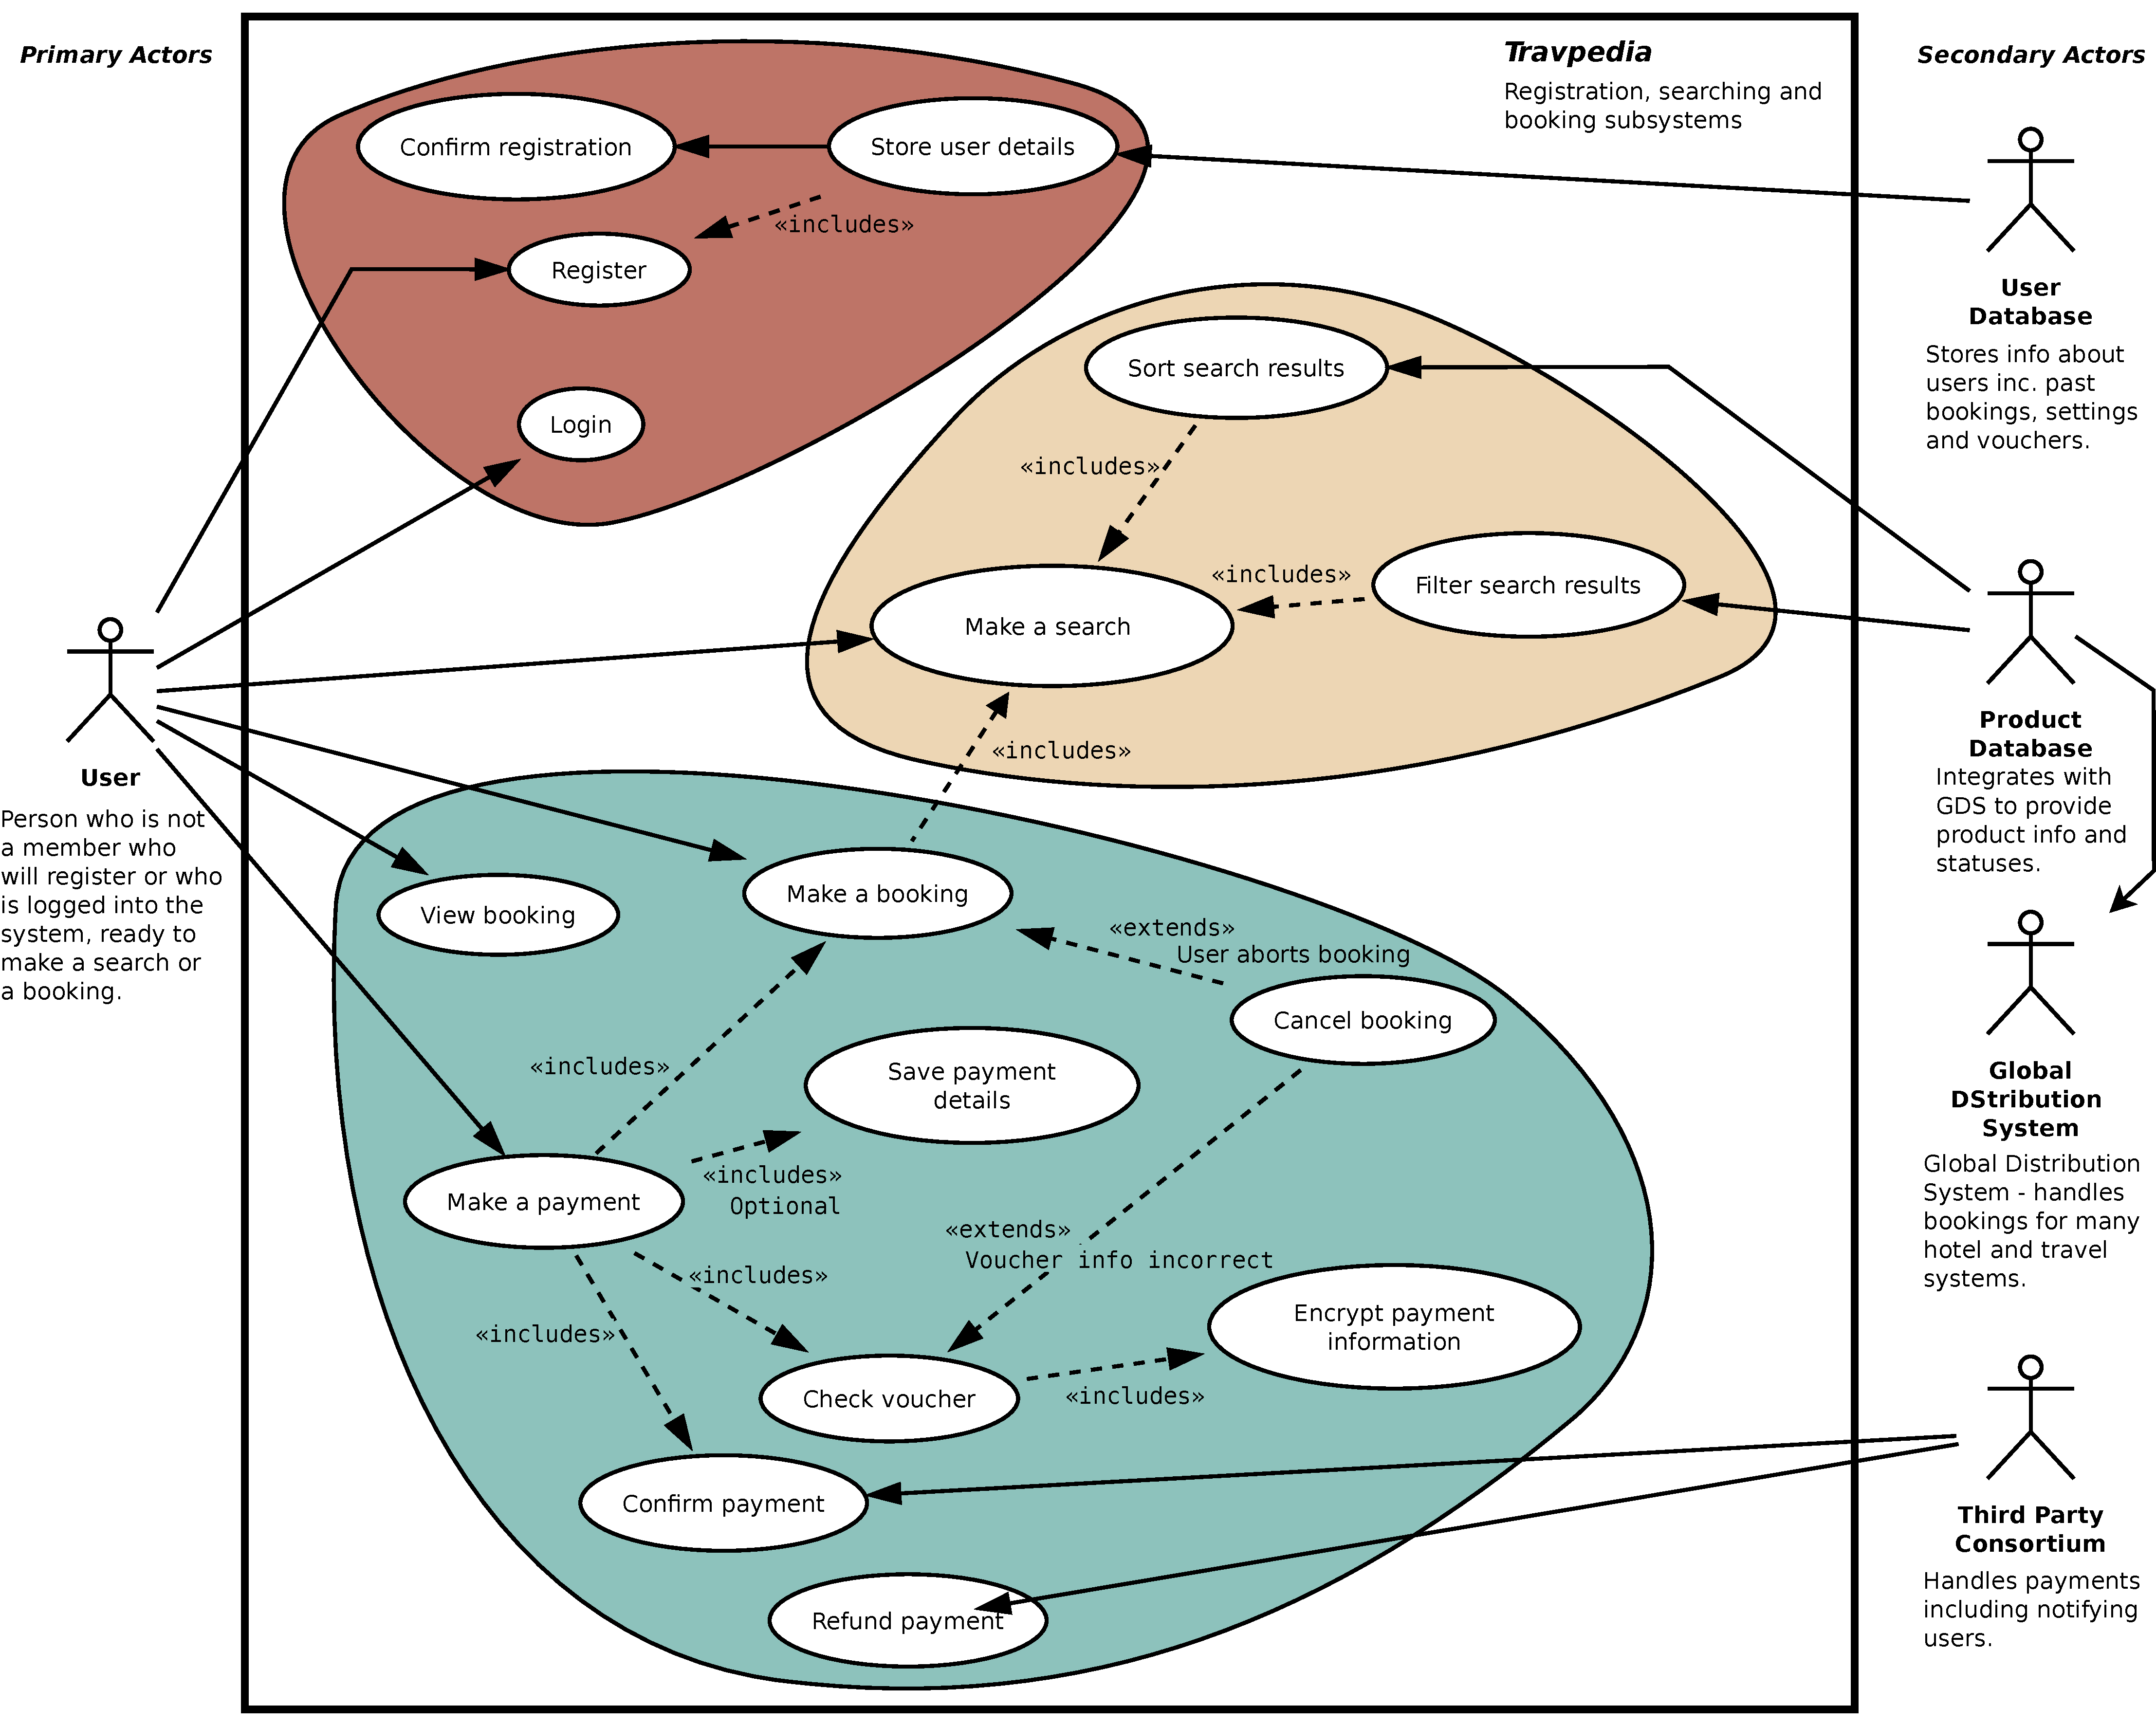
\includegraphics[angle=90,width=1.06\linewidth]{../UseCaseDiagram/UseCaseDiagram.pdf}}%
	\caption{Use case diagram}
\end{figure}
\tablewidth

% {{{
\hspace{-4.2cm}
\begin{minipage}[h][][s]{\linewidth}
	\section{Detailing a Use Case}
	\subsection{Use Case: Register}
\end{minipage}

\marginhead{\textbf{Actors}}
\begin{itemize}
	\item UserAccount (primary actor)
	\item UserDatabase (secondary actor)
\end{itemize}
\noindent\rule{\textwidth}{0.6pt}

\marginhead{\textbf{Pre-conditions}}
\begin{enumerate}
	\item User does not have an account with Travpedia
	\item User has an email address
\end{enumerate}
\noindent\rule{\textwidth}{0.6pt}

\marginhead{\textbf{Flow of events (Success Scenario)}}
\begin{enumerate}
	\item User opens the Travpedia website
	\item User is on the homepage and clicks ``Create an Account'' link
	\item The system presents the user with an interface with empty fields
		asking for the following details:
		\begin{itemize}
			\item Name
			\item Email Address
			\item Password
			\item Confirm Password
		\end{itemize}
	\item User fills these fields in and clicks ``Next''
	\item User then has the option to provide their mobile number and tick
		``please text and email me with Travpedia deals and promotional
		offers'' if they wish to receive this service
	\item User ticks ``I have read and agree to the Terms and Conditions''
	\item User clicks ``Create Account'' button. If any details are invalid
		or a field has not been filled, the user will be shown an error
		message and asked to re-enter their information
	\item The system validates the users details and sends a confirmation
		email to the users email address
	\item The system displays a message telling the user that they should
		have received a confirmation email and that they should open this
		email to verify their email address
	\item User opens the confirmation email and clicks on the link to
		verify their email address
	\item The system redirects them back to Travpedia website and informs
		the user that their registration was successful
\end{enumerate}
\noindent\rule{\textwidth}{0.6pt}

\marginhead{\textbf{Post-conditions}}
\begin{enumerate}
	\item Details are stored in the user database and backed up
	\item The user is now registered and is signed in
	\item The user can now search and make a booking
\end{enumerate}
\noindent\rule{\textwidth}{0.6pt}

\marginpar{\textbf{Scenarios}}
\begin{enumerate}
	\item User forgets to tick the box confirming they have read and agree
		to the terms and conditions – cannot proceed to next page
	\item User does not confirm their email address, their registration is
		incomplete
	\item User leaves the interface before clicking ``Create Account'',
		registration is incomplete
\end{enumerate}
\noindent\rule{\textwidth}{0.6pt}

\marginhead{\textbf{Additional Notes}}
The user has the opportunity to update their profile by going into their
account, here they can specify travel and hotel preferences.

\noindent\rule{\textwidth}{0.6pt}
%}}}
%{{{

\vspace{4ex}
\hspace{-4.2cm}
\begin{minipage}[h][][s]{\linewidth}
	\subsection{Use Case: Make a Booking (Hotel Only)}
\end{minipage}

\marginhead{\textbf{Actors}}
\begin{itemize}
	\item UserAccount (primary actor)
	\item User Database  (secondary actor)
	\item Product Database  (secondary actor)
	\item Third Party Consortium (secondary actor)
\end{itemize}
\noindent\rule{\textwidth}{0.6pt}

\marginhead{\textbf{Pre-conditions}}
\begin{enumerate}
	\item User is registered with Travpedia
	\item User has signed in
\end{enumerate}
\noindent\rule{\textwidth}{0.6pt}

\marginhead{\textbf{Flow of events (Success Scenario)}}
\begin{enumerate}
	\item User is on the homepage where they can begin entering their
		search criteria
	\item User ticks ``Accommodation''. Other options include:
		\begin{itemize}
			\item Travel
			\item Package Holiday
		\end{itemize}
	\item The interface changes slightly to accommodate booking a hotel
		only, the following details are required:
		\begin{itemize}
			\item Destination/Hotel name (User can enter postcode, city,
				region or specific hotel)
			\item Check in date (link to a calendar)
			\item Check out date (link to a calendar)
			\item How many rooms
			\item Target price range
		\end{itemize}
	\item User clicks ``Search''
	\item The system presents the user with a list of available hotels, who
		have subscribed to Travpedia, matching their search criteria
	\item User browses the search results. Can filter by price and star
		rating and sort by price, review score and star rating
	\item User click on the hotel they would like to book
	\item The system presents the user with a more detailed view of the
		hotel including photos
	\item User selects the number of room they require
	\item User clicks ``Book Now''
	\item The system presents the user with an interface with empty fields
		asking for various payment details:
		\begin{itemize}
			\item Name on card
			\item Billing address
			\item Card type
			\item Card number
			\item Expiry date
			\item Security number
			\item Voucher code (if entered, the system will reload the page
				displaying the new price to pay)
			\item Option to have Travpedia save payment  details
		\end{itemize}
	\item User fills in all the fields
	\item User ticks to agree to terms and conditions
	\item User clicks ``Pay Now''
	\item User is presented with another screen summarising booking and
		payments details
	\item User clicks ``Confirm''
	\item The transaction information is securely passed by the system to
		the credit/debit card consortium where the user''s payment details
		are validated
	\item The booking is processed and handled by the GDS
	\item The system redirects the users to a page thanking them for their
		booking
\end{enumerate}
\noindent\rule{\textwidth}{0.6pt}

\marginhead{\textbf{Post-conditions}}
\begin{enumerate}
	\item User receives a confirmation email
	\item Details of the booking are stored in the user database –
		behaviour of user is used to determine future promotional offers
		and recommendations
	\item Payment details are securely stored in the user database (if user
		selects to save payment details)
	\item Details of the booking are available to view in ``Manage
		Bookings''
\end{enumerate}
\noindent\rule{\textwidth}{0.6pt}

\marginhead{\textbf{Scenarios}}
\begin{enumerate}
	\item The destination or hotel name the user has specified produces no
		matches
	\item User enters the incorrect account number  – consortium confirms
		this, system generates an error message
	\item User may think booking is complete after clicking ``Pay Now'' –
		leaves website before clicking ``Confirm'' – booking is incomplete
	\item When user clicks ``Confirm'', the system loads for several minutes
		and eventually times out – booking is incomplete
\end{enumerate}
\noindent\rule{\textwidth}{0.6pt}
%}}}
%{{{

\vspace{4ex}
\hspace{-4.2cm}
\begin{minipage}[h][][s]{\linewidth}
	\subsection{Use Case: Make a Booking (Travel by Plane)}
\end{minipage}

\marginhead{\textbf{Actors}}
\begin{itemize}
	\item UserAccount (primary actor)
	\item User Database  (secondary actor)
	\item Product Database  (secondary actor)
	\item Third Party Consortium (secondary actor)
\end{itemize}
\noindent\rule{\textwidth}{0.6pt}

\marginhead{\textbf{Pre-conditions}}
\begin{enumerate}
	\item User is registered with Travpedia
	\item User has signed in
\end{enumerate}
\noindent\rule{\textwidth}{0.6pt}

\marginhead{\textbf{Flow of events (Success Scenario)}}
\begin{enumerate}
	\item User is on the homepage where they can begin entering their search
		criteria
	\item User ticks ``Travel''. Other options include:
	\begin{itemize}
		\item Accommodation
		\item Package Holiday
	\end{itemize}
	\item The interface changes slightly to accommodate booking a journey
	\item User ticks ``One way'',  the following details are required:
	\begin{itemize}
		\item Type (of transport)
		\item Date (link to calendar)
		\item Start location
		\item End location
		\item Number of
	\end{itemize}
	\item User clicks ``Search''
	\item The system presents the user with a list of available flights, whose
		airline companies have subscribed to Travpedia, matching their search
		criteria
	\item User browses the search results. Can filter by price range and sort
		by price and departure time
	\item User clicks on the journey they would like to book
	\item The system presents the user with a more detailed view of the flight
	\item User selects how many items of luggage they wish to take on the
		flight
	\item User clicks ``Book Now''
	\item The system presents the user with an interface with the total price
		and empty fields asking for various payment details:
	\begin{itemize}
		\item Passport number
		\item Passport issue date
		\item Name on card
		\item Billing address
		\item Card type
		\item Card number
		\item Expiry date
		\item Security number
		\item Voucher code (if entered, the system will reload the page
			displaying the new price to pay)
		\item Option to have Travpedia save payment  details
	\end{itemize}
	\item User fills in all the fields
	\item User ticks to agree to terms and conditions
	\item User clicks ``Pay Now''
	\item User is presented with another screen summarising booking and
		payments details
	\item User clicks ``Confirm''
	\item The transaction information is securely passed by the system to the
		credit/debit card consortium where the user''s payment details are
		validated
	\item The booking is processed and handled by the GDS
	\item The system redirects the users to a page thanking them for their
		booking
\end{enumerate}
\noindent\rule{\textwidth}{0.6pt}

\marginhead{\textbf{Post-conditions}}
\begin{enumerate}
	\item User receives a confirmation email
	\item Details of the booking are stored in the user database – behaviour of
		user is used to determine future promotional offers and recommendations
	\item Payment details are securely stored in the user database (if user
		selects to save payment details)
	\item Details of the booking are available to view in ``Manage Bookings''
	\item Airline company is notified of the booking
\end{enumerate}
\noindent\rule{\textwidth}{0.6pt}

\marginhead{\textbf{Scenarios}}
\begin{enumerate}
	\item The search criteria produces no results
	\item User enters an invalid passport number - error message
\end{enumerate}
\noindent\rule{\textwidth}{0.6pt}
%}}}
%{{{

\vspace{4ex}
\hspace{-4.2cm}
\begin{minipage}[h][][s]{\linewidth}
	\subsection{Use Case: Cancel a Booking}
\end{minipage}

\marginhead{\textbf{Actors}}
\begin{itemize}
	\item UserAccount (primary actor)
	\item Product Database (secondary actor)
	\item User Database (secondary actor)
\end{itemize}
\noindent\rule{\textwidth}{0.6pt}

\marginhead{\textbf{Pre-conditions}}
\begin{enumerate}
	\item User is registered
	\item User is logged in
	\item User has made a booking
	\item The terms and conditions of the booking in question specify that
		cancellations are permitted
\end{enumerate}
\noindent\rule{\textwidth}{0.6pt}

\marginhead{\textbf{Flow of events (Success Scenario)}}
\begin{enumerate}
	\item User clicks ``Manage Bookings'' on the website''s homepage
	\item The system directs the user to a page showing their past and current
		bookings
	\item User clicks on the booking they wish to cancel
	\item The system shows the booking in more detail with an option to cancel
		the booking
	\item User clicks ``Cancel booking''
	\item User is asked to confirm that they are sure they want to cancel the
		booking
	\item User clicks ``Confirm Cancellation''
	\item This information is relayed to the credit/debit card consortium which
		will handle the refund
	\item The system redirects the user to a page confirming their cancellation
		was successful
\end{enumerate}
\noindent\rule{\textwidth}{0.6pt}

\marginhead{\textbf{Post-conditions}}
\begin{enumerate}
	\item Hotel company is notified of the cancellation
	\item User receives email confirmation of cancellation
	\item Booking is removed from the user''s account in ``Manage Bookings''
	\item Both databases are updated of changes
	\item User receives appropriate refund
\end{enumerate}
\noindent\rule{\textwidth}{0.6pt}

\marginhead{\textbf{Scenarios}}
\begin{enumerate}
	\item User disputes a no refund policy – not possible using website. User
		must contact the company directly
	\item User leaves the website after clicking ``Cancel Booking'' – User has
		not clicked ``Confirm Cancellation'' – Booking has not been cancelled
\end{enumerate}
\noindent\rule{\textwidth}{0.6pt}
%}}}

\restoregeometry

\section{Activity Diagram}

The activity diagram models the scenario for the user searching for and making
an accommodation booking.

\begin{figure}[h!]
	\centering
	\makebox[\textwidth][c]{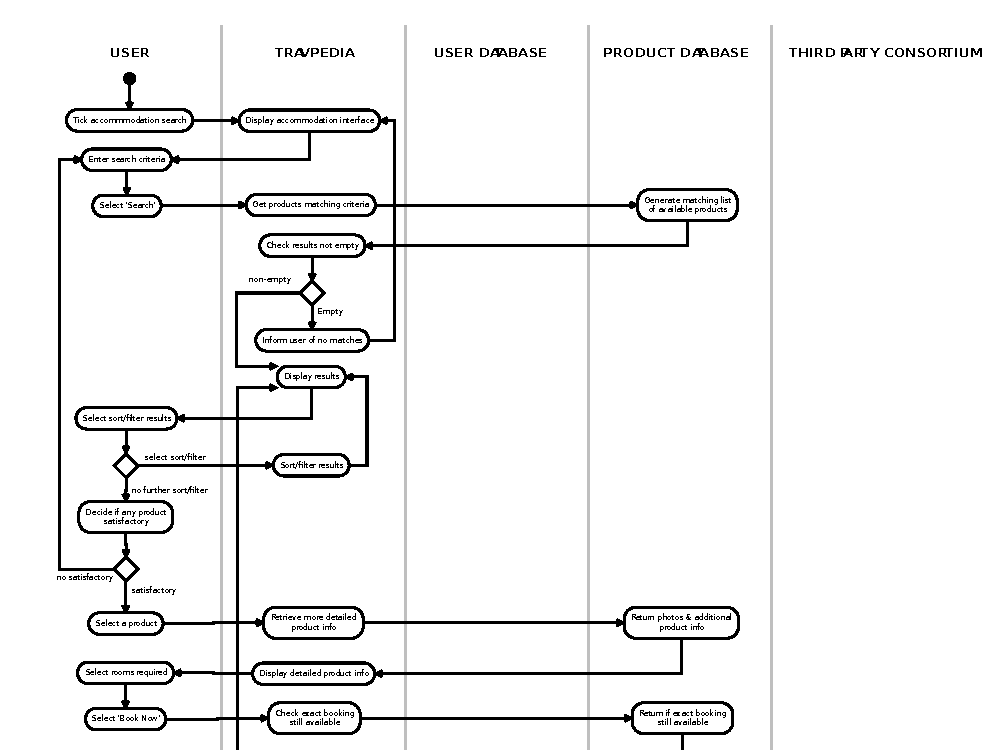
\includegraphics[angle=90,width=\linewidth]{../ActivityDiagram/ActivityDiagram_top.pdf}}%
	\caption{Activity diagram}
\end{figure}
\begin{figure}[h!]
	\centering
	\makebox[\textwidth][c]{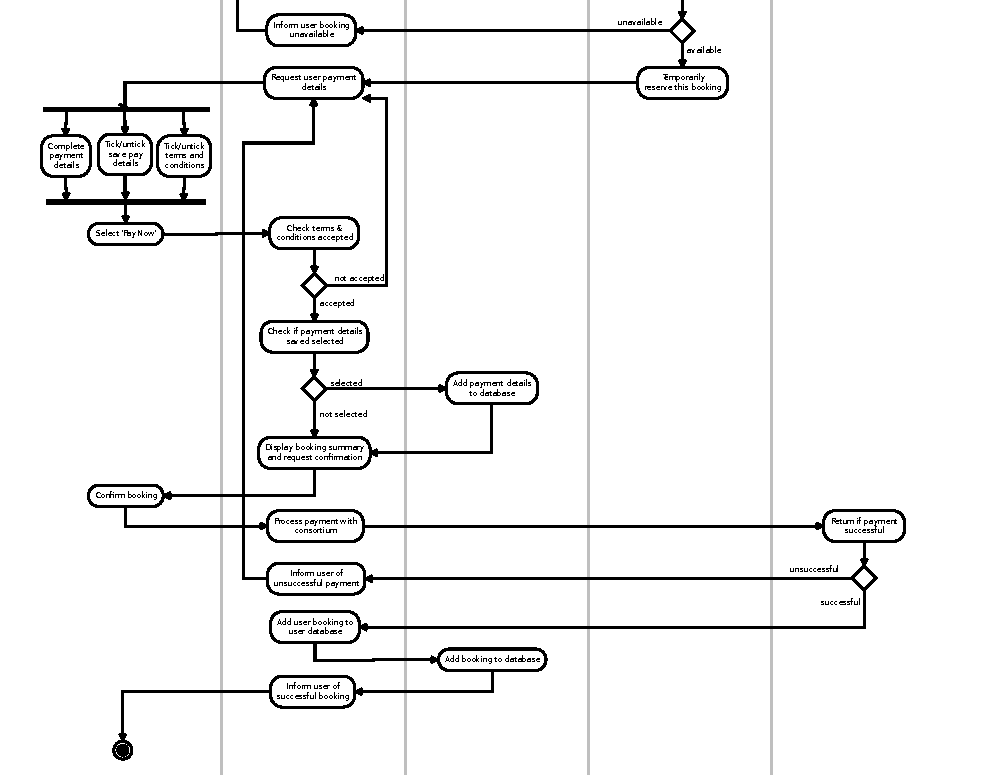
\includegraphics[angle=90,width=\linewidth]{../ActivityDiagram/ActivityDiagram_bottom.pdf}}%
	\caption{Activity diagram}
\end{figure}
\clearpage

\section{Class Analysis}

\subsection{Responsibility-Driven Analysis }

\anoun{Travpedia} is an online travel and accommodation \anoun{booking system}.

\emph{Travel and accommodation companies are able to subscribe to Travpedia for
a monthly subscription cost of £200 plus an initial £50 joining fee. This
subscription allows the company to offer their products on the Travpedia
website where they can be purchased by visiting users.}

\anoun{Products} that are \averb{advertised} on the Travpedia \anoun{website}
include \anoun{accommodation}, \anoun{package holidays} and \anoun{travel} by
\anoun{air}, \anoun{rail} and \anoun{sea,}

Visitors to the website, after \averb{registering} an \anoun{account}, are able
to \averb{search} for all available products \averb{offered} by these
subscribed \anoun{companies}. They are able to search with a number of
\anoun{criteria} including \anoun{type of product}, \anoun{location},
\anoun{date} and \anoun{price}. Users can then view these \anoun{search
results} and \averb{book} and \averb{pay} for products through the website.
Users may also \averb{rate} and \averb{review} individual products and services
that they have \averb{purchased}. A product gains a review score based on
these ratings. This review rating system provides further search criteria
whereby a user can \averb{filter} search results by \anoun{review score}.

\anoun{Payments} made by both subscribing companies and users are
\averb{handled} online by a third party \anoun{consortium}.
\anoun{Subscribers} must pay by \anoun{debit} or \anoun{credit card} while
users have the additional option of paying with gift \anoun{vouchers} offered
by Travpedia.

Users are able to \averb{view }\anoun{bookings} they have made and, where
possible, \averb{cancel} these bookings and \averb{receive} a \anoun{refund}
via the third party consortium.

\emph{Travpedia disseminates advertisements and promotional offers to users
based on previous patterns of use and previous purchases.  These personalised
offering are sent to mobile phones through SMS and email accounts.}

Users may \averb{opt out} of receiving phone and email \anoun{alerts}.

\subsection{CRC Analysis}

Responsibilities of a class are things it knows and things it does. Terminology
used here:
\begin{description}
	\item[Has] this is required
	\item[May have] this is optional
	\item[Maintains] used where class contains a collection of zero more objects
\end{description}

\begin{center}
\renewcommand{\arraystretch}{1.5}
\begin{tabu}{p{8cm} | p{3cm}}
	\multicolumn{2}{l}{\cellcolor{blue!25}\textbf{User Account}} \\
	\toprule
	\multicolumn{2}{l}{\emph{Superclass:}} \\
	\midrule
	\multicolumn{2}{l}{\emph{Subclass:}} \\
	\midrule
	\emph{Responsibilities}: & \emph{Collaborators:} \\
	\midrule
	Maintains user profile information & \\
	Maintains stored payment method information & \\
	Maintains user preferences & \\
	Maintains a collection of past and current bookings & Booking \\
	\bottomrule
\end{tabu}
\end{center}

\begin{center}
\renewcommand{\arraystretch}{1.5}
\begin{tabu}{p{8cm} | p{3cm}}
	\multicolumn{2}{l}{\cellcolor{blue!25}\textbf{Product (Abstract)}} \\
	\toprule
	\multicolumn{2}{l}{\emph{Superclass:}} \\
	\midrule
	\multicolumn{2}{l}{\emph{Subclass:} PackageHoliday, Accommodation, Journey} \\
	\midrule
	\emph{Responsibilities}: & \emph{Collaborators:} \\
	\midrule
	A superclass maintaining information about a journey or accommodation product
	& Journey \newline
		PackageHoliday \newline
		Accommodation \\
	Has a product reference & \\
	Has a price & \\
	\bottomrule
\end{tabu}
\end{center}

\begin{center}
\renewcommand{\arraystretch}{1.5}
\begin{tabu}{p{8cm} | p{3cm}}
	\multicolumn{2}{l}{\cellcolor{blue!25}\textbf{Journey}} \\
	\toprule
	\multicolumn{2}{l}{\emph{Superclass:} Product} \\
	\midrule
	\multicolumn{2}{l}{\emph{Subclass:}} \\
	\midrule
	\emph{Responsibilities}: & \emph{Collaborators:} \\
	\midrule
	Maintains information about a particular journey: dates, start and end
	location & \\
	Has a transport type & \\
	Is bookable & \\
	\bottomrule
\end{tabu}
\end{center}

\begin{center}
\renewcommand{\arraystretch}{1.5}
\begin{tabu}{p{8cm} | p{3cm}}
	\multicolumn{2}{l}{\cellcolor{blue!25}\textbf{Accommodation}} \\
	\toprule
	\multicolumn{2}{l}{\emph{Superclass:} Product} \\
	\midrule
	\multicolumn{2}{l}{\emph{Subclass:}} \\
	\midrule
	\emph{Responsibilities}: & \emph{Collaborators:} \\
	\midrule
	Maintains details about the accommodation & \\
	Maintains information & \\
	Is able to calculate its review score & \\
	Has a star rating & \\
	Is reviewable & Review \\
	\bottomrule
\end{tabu}
\end{center}

\begin{center}
\renewcommand{\arraystretch}{1.5}
\begin{tabu}{p{8cm} | p{3cm}}
	\multicolumn{2}{l}{\cellcolor{blue!25}\textbf{Package Holiday}} \\
	\toprule
	\multicolumn{2}{l}{\emph{Superclass:} Product} \\
	\midrule
	\multicolumn{2}{l}{\emph{Subclass:}} \\
	\midrule
	\emph{Responsibilities}: & \emph{Collaborators:} \\
	\midrule
	Maintains information about a PackageHoliday & \\
	Is reviewable & \\
	Maintains a collection of reviews & Review \\
	\bottomrule
\end{tabu}
\end{center}

\begin{center}
\renewcommand{\arraystretch}{1.5}
\begin{tabu}{p{8cm} | p{3cm}}
	\multicolumn{2}{l}{\cellcolor{blue!25}\textbf{Booking}} \\
	\toprule
	\multicolumn{2}{l}{\emph{Superclass:}} \\
	\midrule
	\multicolumn{2}{l}{\emph{Subclass:}} \\
	\midrule
	\emph{Responsibilities}: & \emph{Collaborators:} \\
	\midrule
	Has one or more Travel Products & Travel Product \\
	Is payable & \\
	Is viewable & \\
	Is cancellable & \\
	\bottomrule
\end{tabu}
\end{center}

\begin{center}
\renewcommand{\arraystretch}{1.5}
\begin{tabu}{p{8cm} | p{3cm}}
	\multicolumn{2}{l}{\cellcolor{blue!25}\textbf{Payment}} \\
	\toprule
	\multicolumn{2}{l}{\emph{Superclass:}} \\
	\midrule
	\multicolumn{2}{l}{\emph{Subclass:}} \\
	\midrule
	\emph{Responsibilities}: & \emph{Collaborators:} \\
	\midrule
	Maintains a collection of Travpedia Vouchers used & Travpedia Voucher \\
	May know details of payment card used & Payment card \\
	May know card authorization code & \\
	Can send itself to payment subsystem & \\
	\bottomrule
\end{tabu}
\end{center}

\begin{center}
\renewcommand{\arraystretch}{1.5}
\begin{tabu}{p{8cm} | p{3cm}}
	\multicolumn{2}{l}{\cellcolor{blue!25}\textbf{Search Results}} \\
	\toprule
	\multicolumn{2}{l}{\emph{Superclass:}} \\
	\midrule
	\multicolumn{2}{l}{\emph{Subclass:}} \\
	\midrule
	\emph{Responsibilities}: & \emph{Collaborators:} \\
	\midrule
	Has criteria & Travel Product \\
	Maintains a collection of Travel Products that satisfy its criteria & \\
	Can sort itself by price or review score & \\
	Can filter itself by price range, review score, board basis or star rating & Review \\
	\bottomrule
\end{tabu}
\end{center}

\begin{center}
\renewcommand{\arraystretch}{1.5}
\begin{tabu}{p{8cm} | p{3cm}}
	\multicolumn{2}{l}{\cellcolor{blue!25}\textbf{Reveiw}} \\
	\toprule
	\multicolumn{2}{l}{\emph{Superclass:}} \\
	\midrule
	\multicolumn{2}{l}{\emph{Subclass:}} \\
	\midrule
	\emph{Responsibilities}: & \emph{Collaborators:} \\
	\midrule
	Maintains all information pertaining &
		Accommodation \newline
		PackageHoliday \\
	\bottomrule
\end{tabu}
\end{center}
\clearpage

\section{First Cut Class Diagram}

The first cut class diagram shows the results of the noun verb analysis that we
performed. Some of the nouns and verbs were not suitable to keep as classes and
methods as they were generic or duplicated. The diagram shows the basic
skeletal structure that will adopted for the system.

\begin{figure}[h!]
	\centering
	\makebox[\textwidth][c]{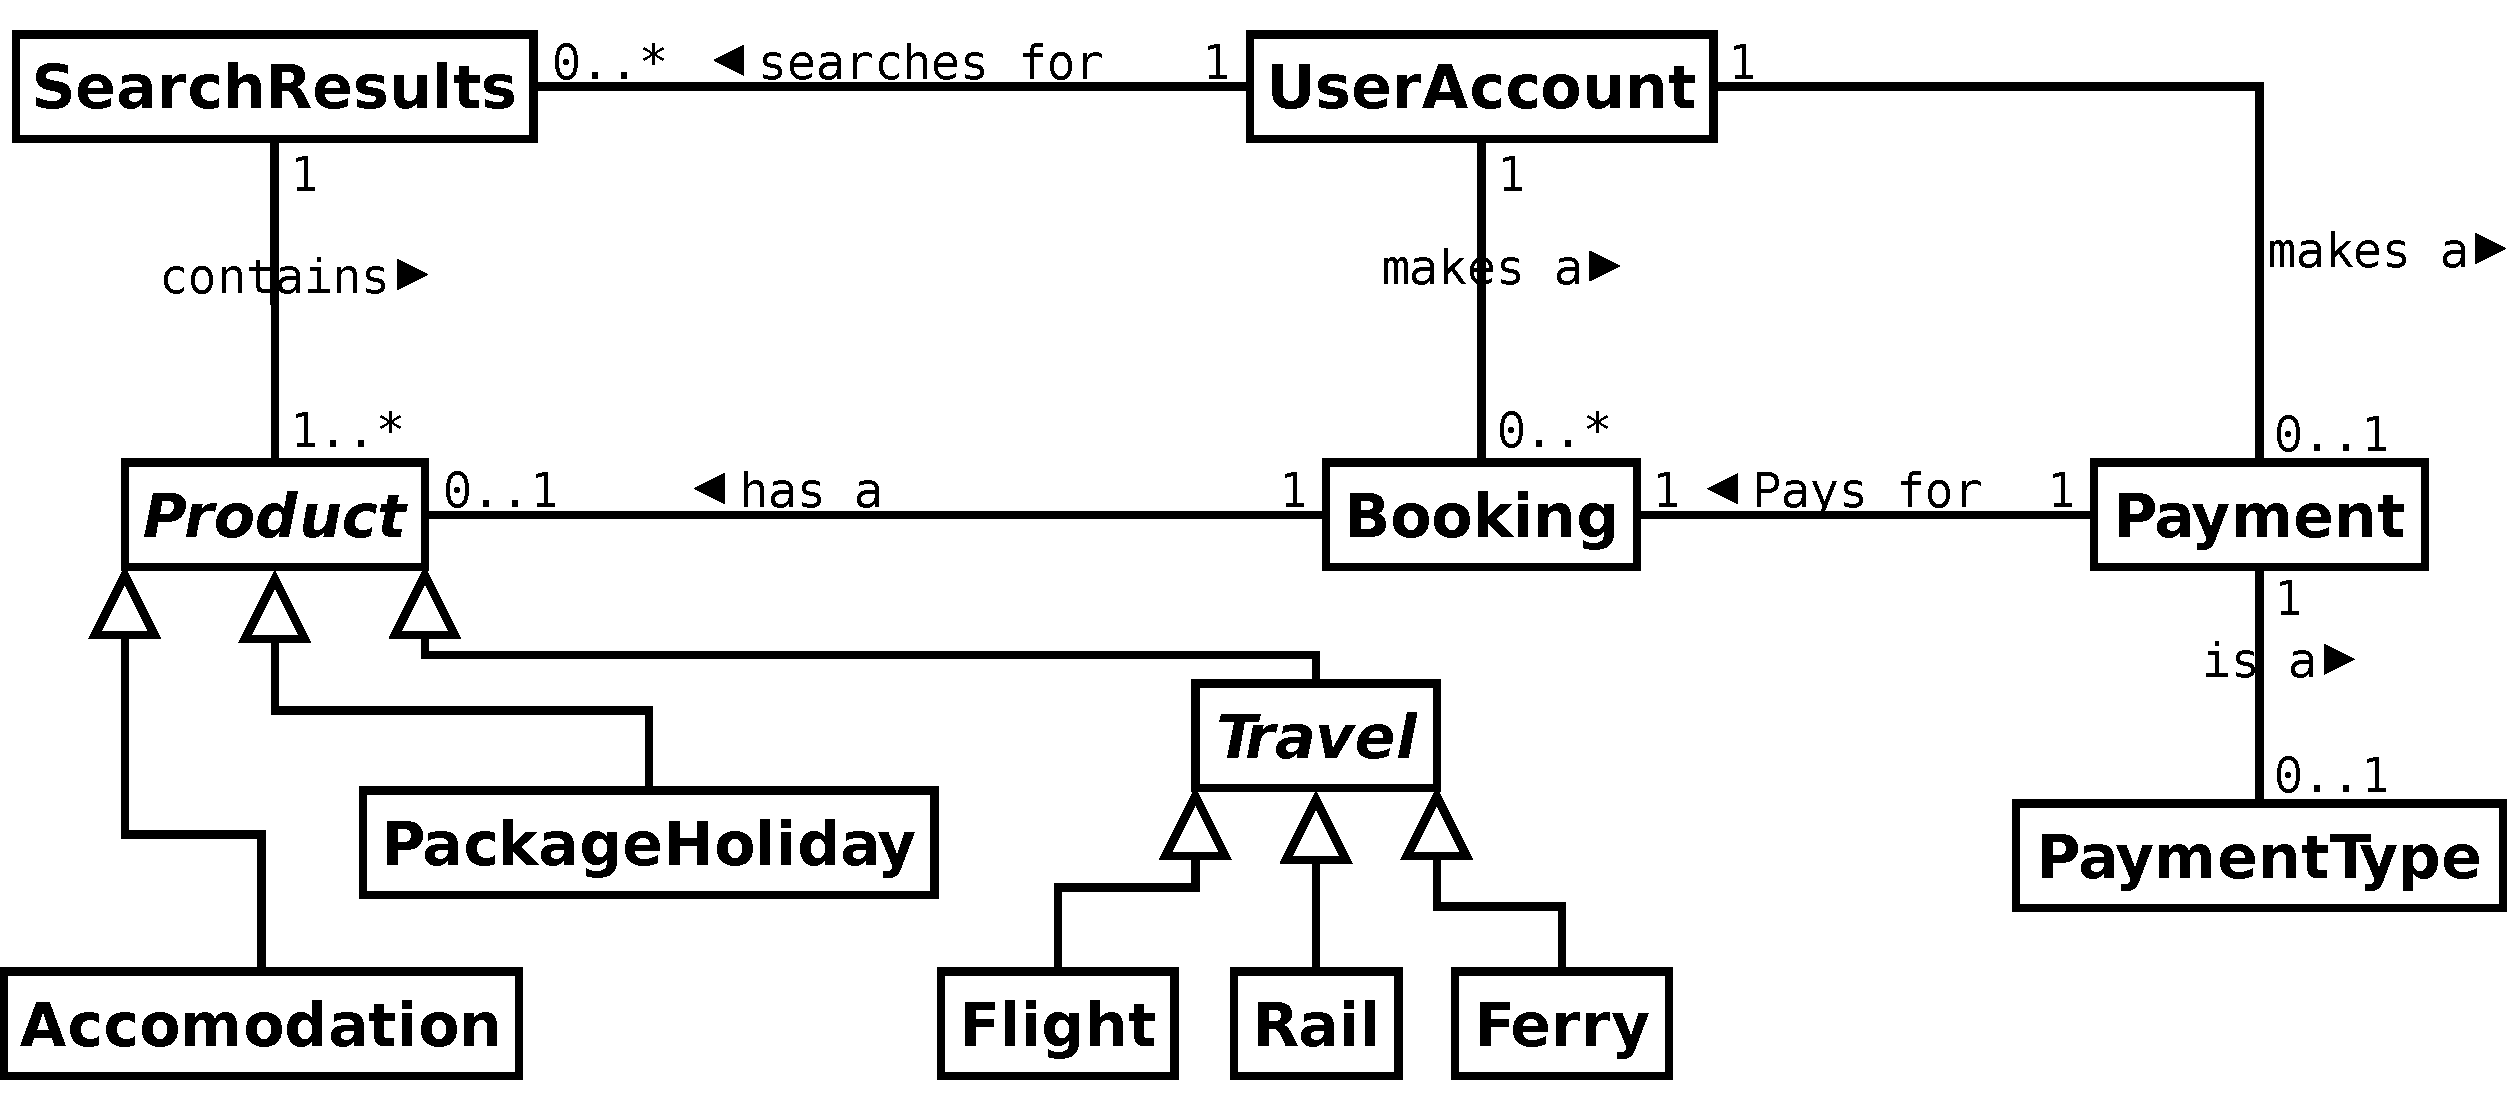
\includegraphics[angle=90,height=0.83\textheight]{../ClassDiagram/FirstCutClass.pdf}}%
	\caption{First cut class diagram}
\end{figure}
\clearpage

\section{Class Diagram}

The class diagram is an extension of the first cut class diagram with methods
and class hierachies included. It is assumed that getters and setters are
included for many of the field variables, but these have been left off for
brevity.

\begin{figure}[h!]
	\centering
	\makebox[\textwidth][c]{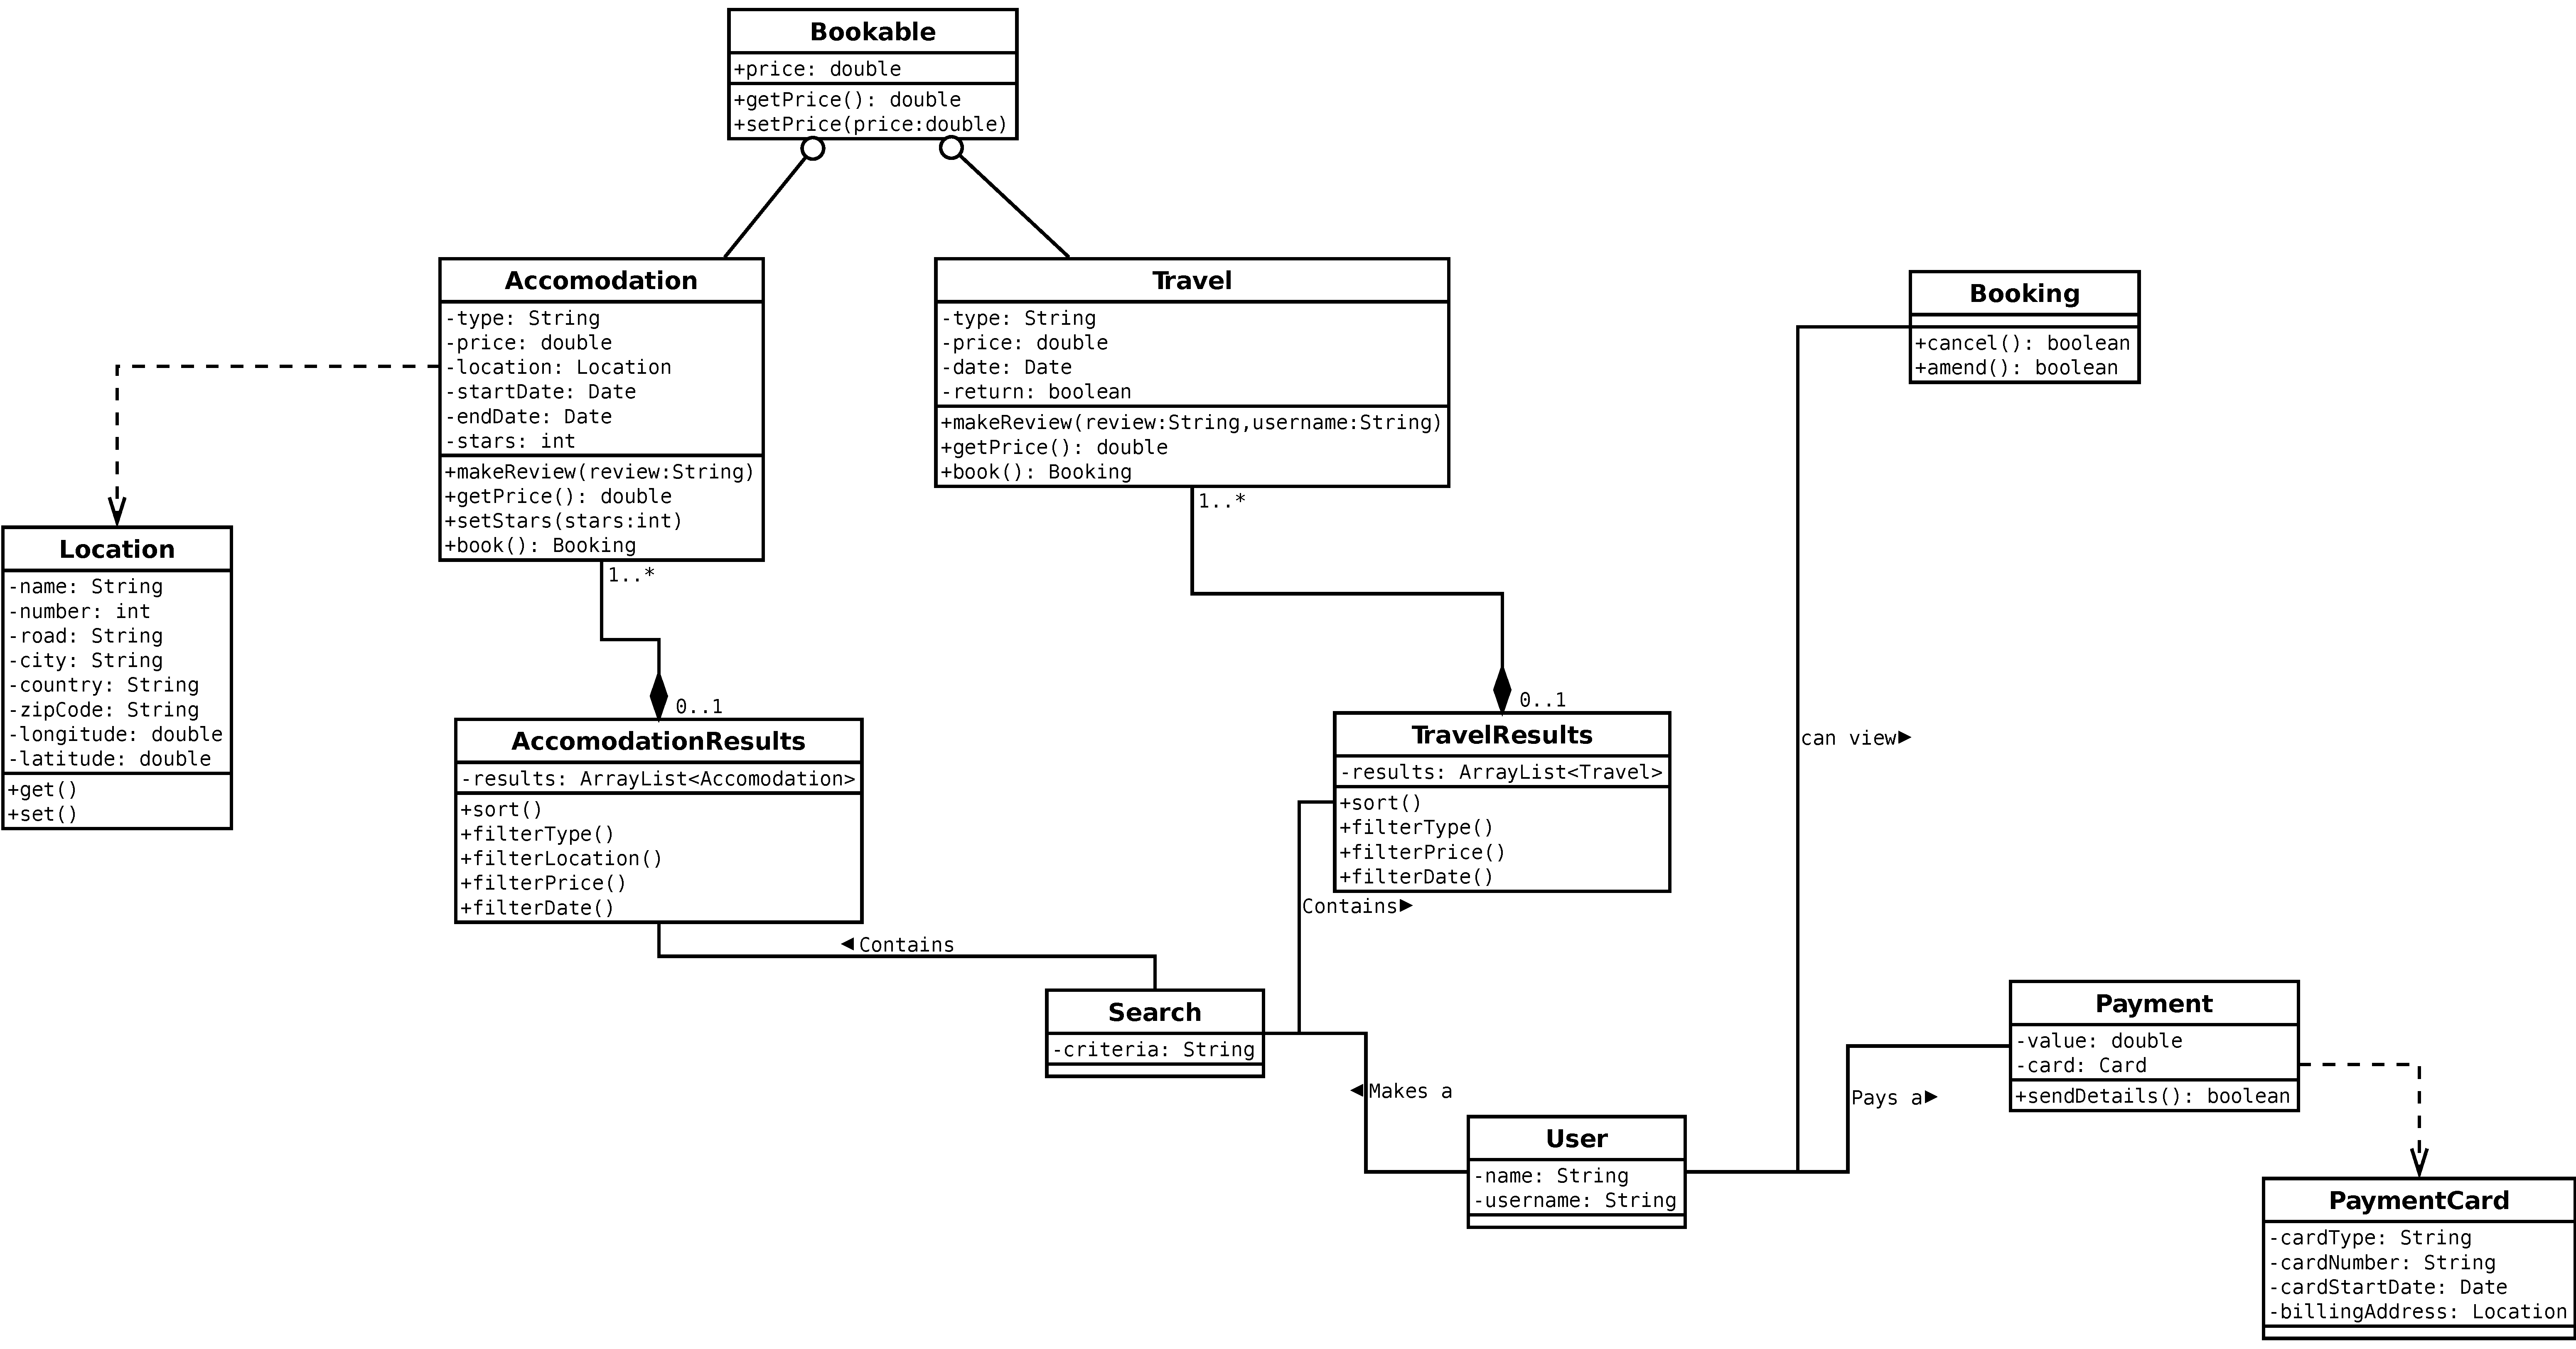
\includegraphics[angle=90,height=0.85\textheight]{../ClassDiagram/ClassDiagram.pdf}}%
	\caption{Class diagram}
\end{figure}
\clearpage

\section{Object Diagram}

The object diagram below relates the following scenario:

\begin{quote}
	A user called Howard Evans wants to book accomodation at a five star hotel
	in London. He wants to pay by card and stay for 5 nights starting on
	Christmas day this year.
\end{quote}

\begin{figure}[h!]
	\centering
	\makebox[\textwidth][c]{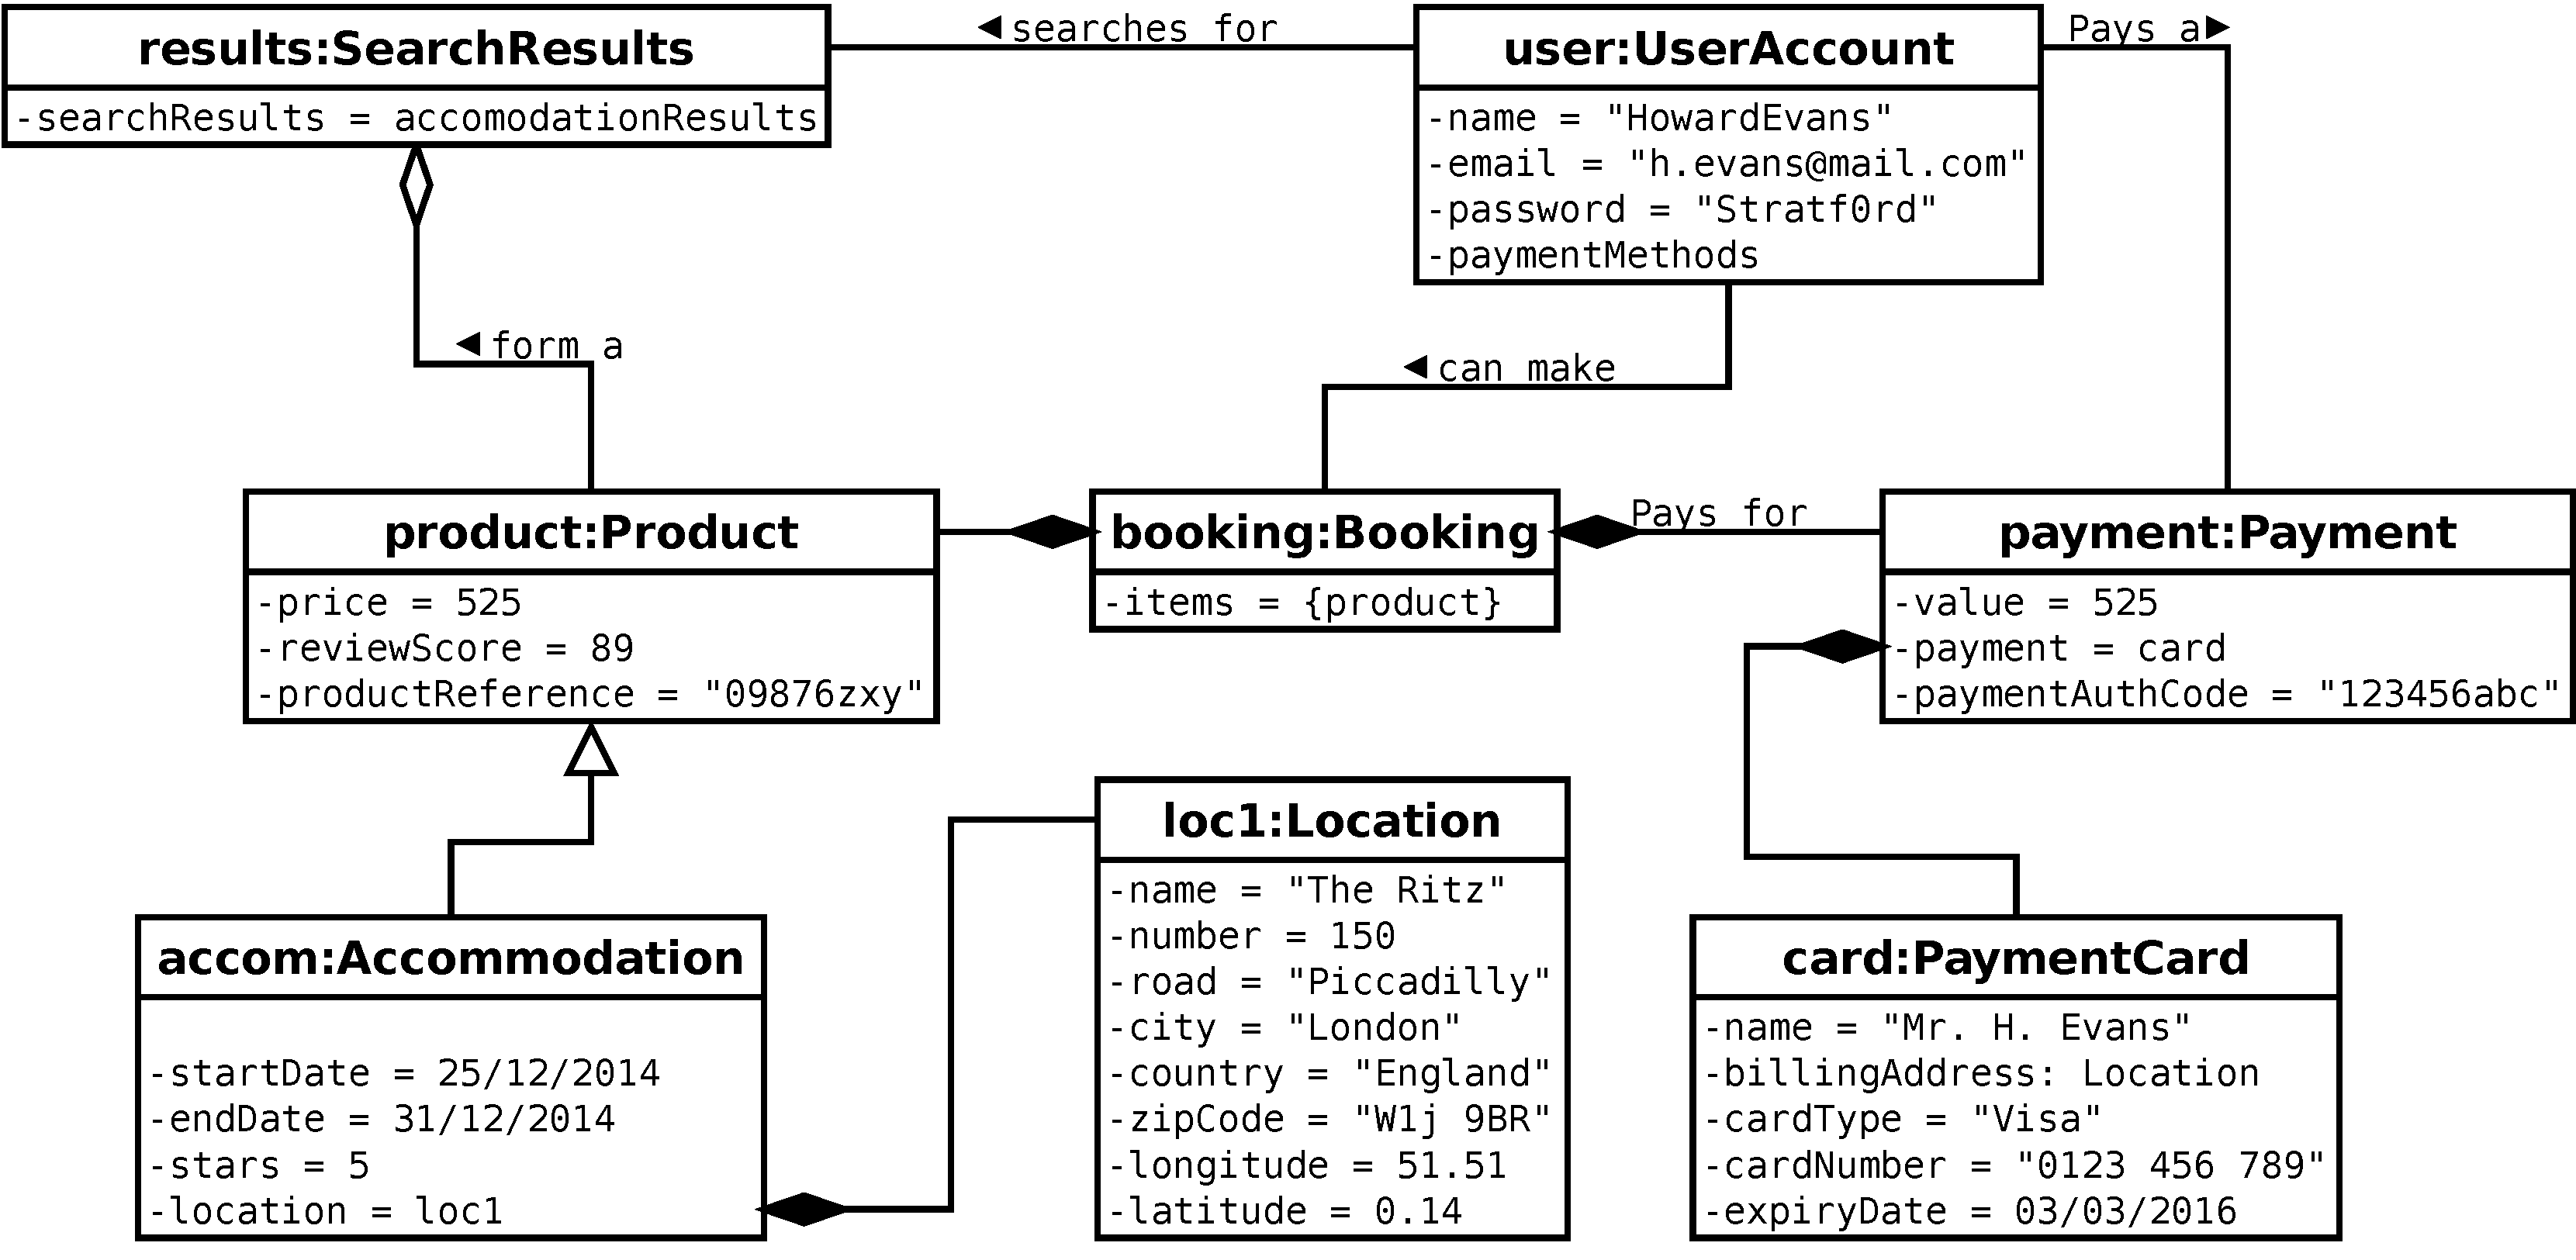
\includegraphics[angle=90,height=0.81\textheight]{../ObjectDiagram/ObjectDiagram.pdf}}%
	\caption{Object diagram}
\end{figure}
\clearpage

\section{Sequence Diagram}
\begin{figure}[h!]
	\centering
	\makebox[\textwidth][c]{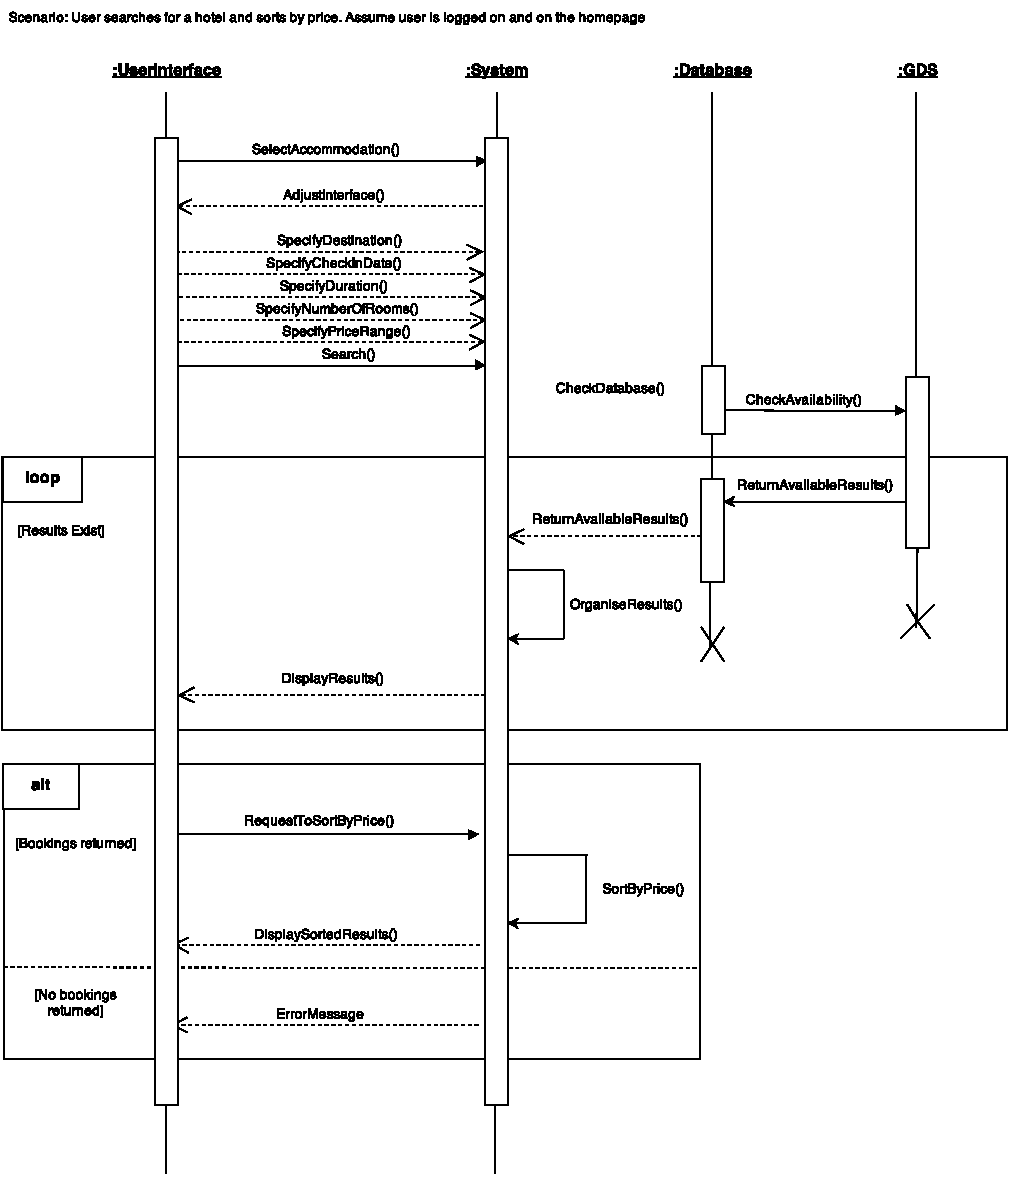
\includegraphics[width=1.2\textwidth]{../SequenceDiagram/SequenceDiagramNonTrival.pdf}}%
	\caption{Sequence diagram}
\end{figure}
\clearpage

\section{State Diagram}

This state diagram, of the searching and booking system, shows the scenario for
the user searching for and making an accommodation booking.

\begin{figure}[h!]
	\centering
	\makebox[\textwidth][c]{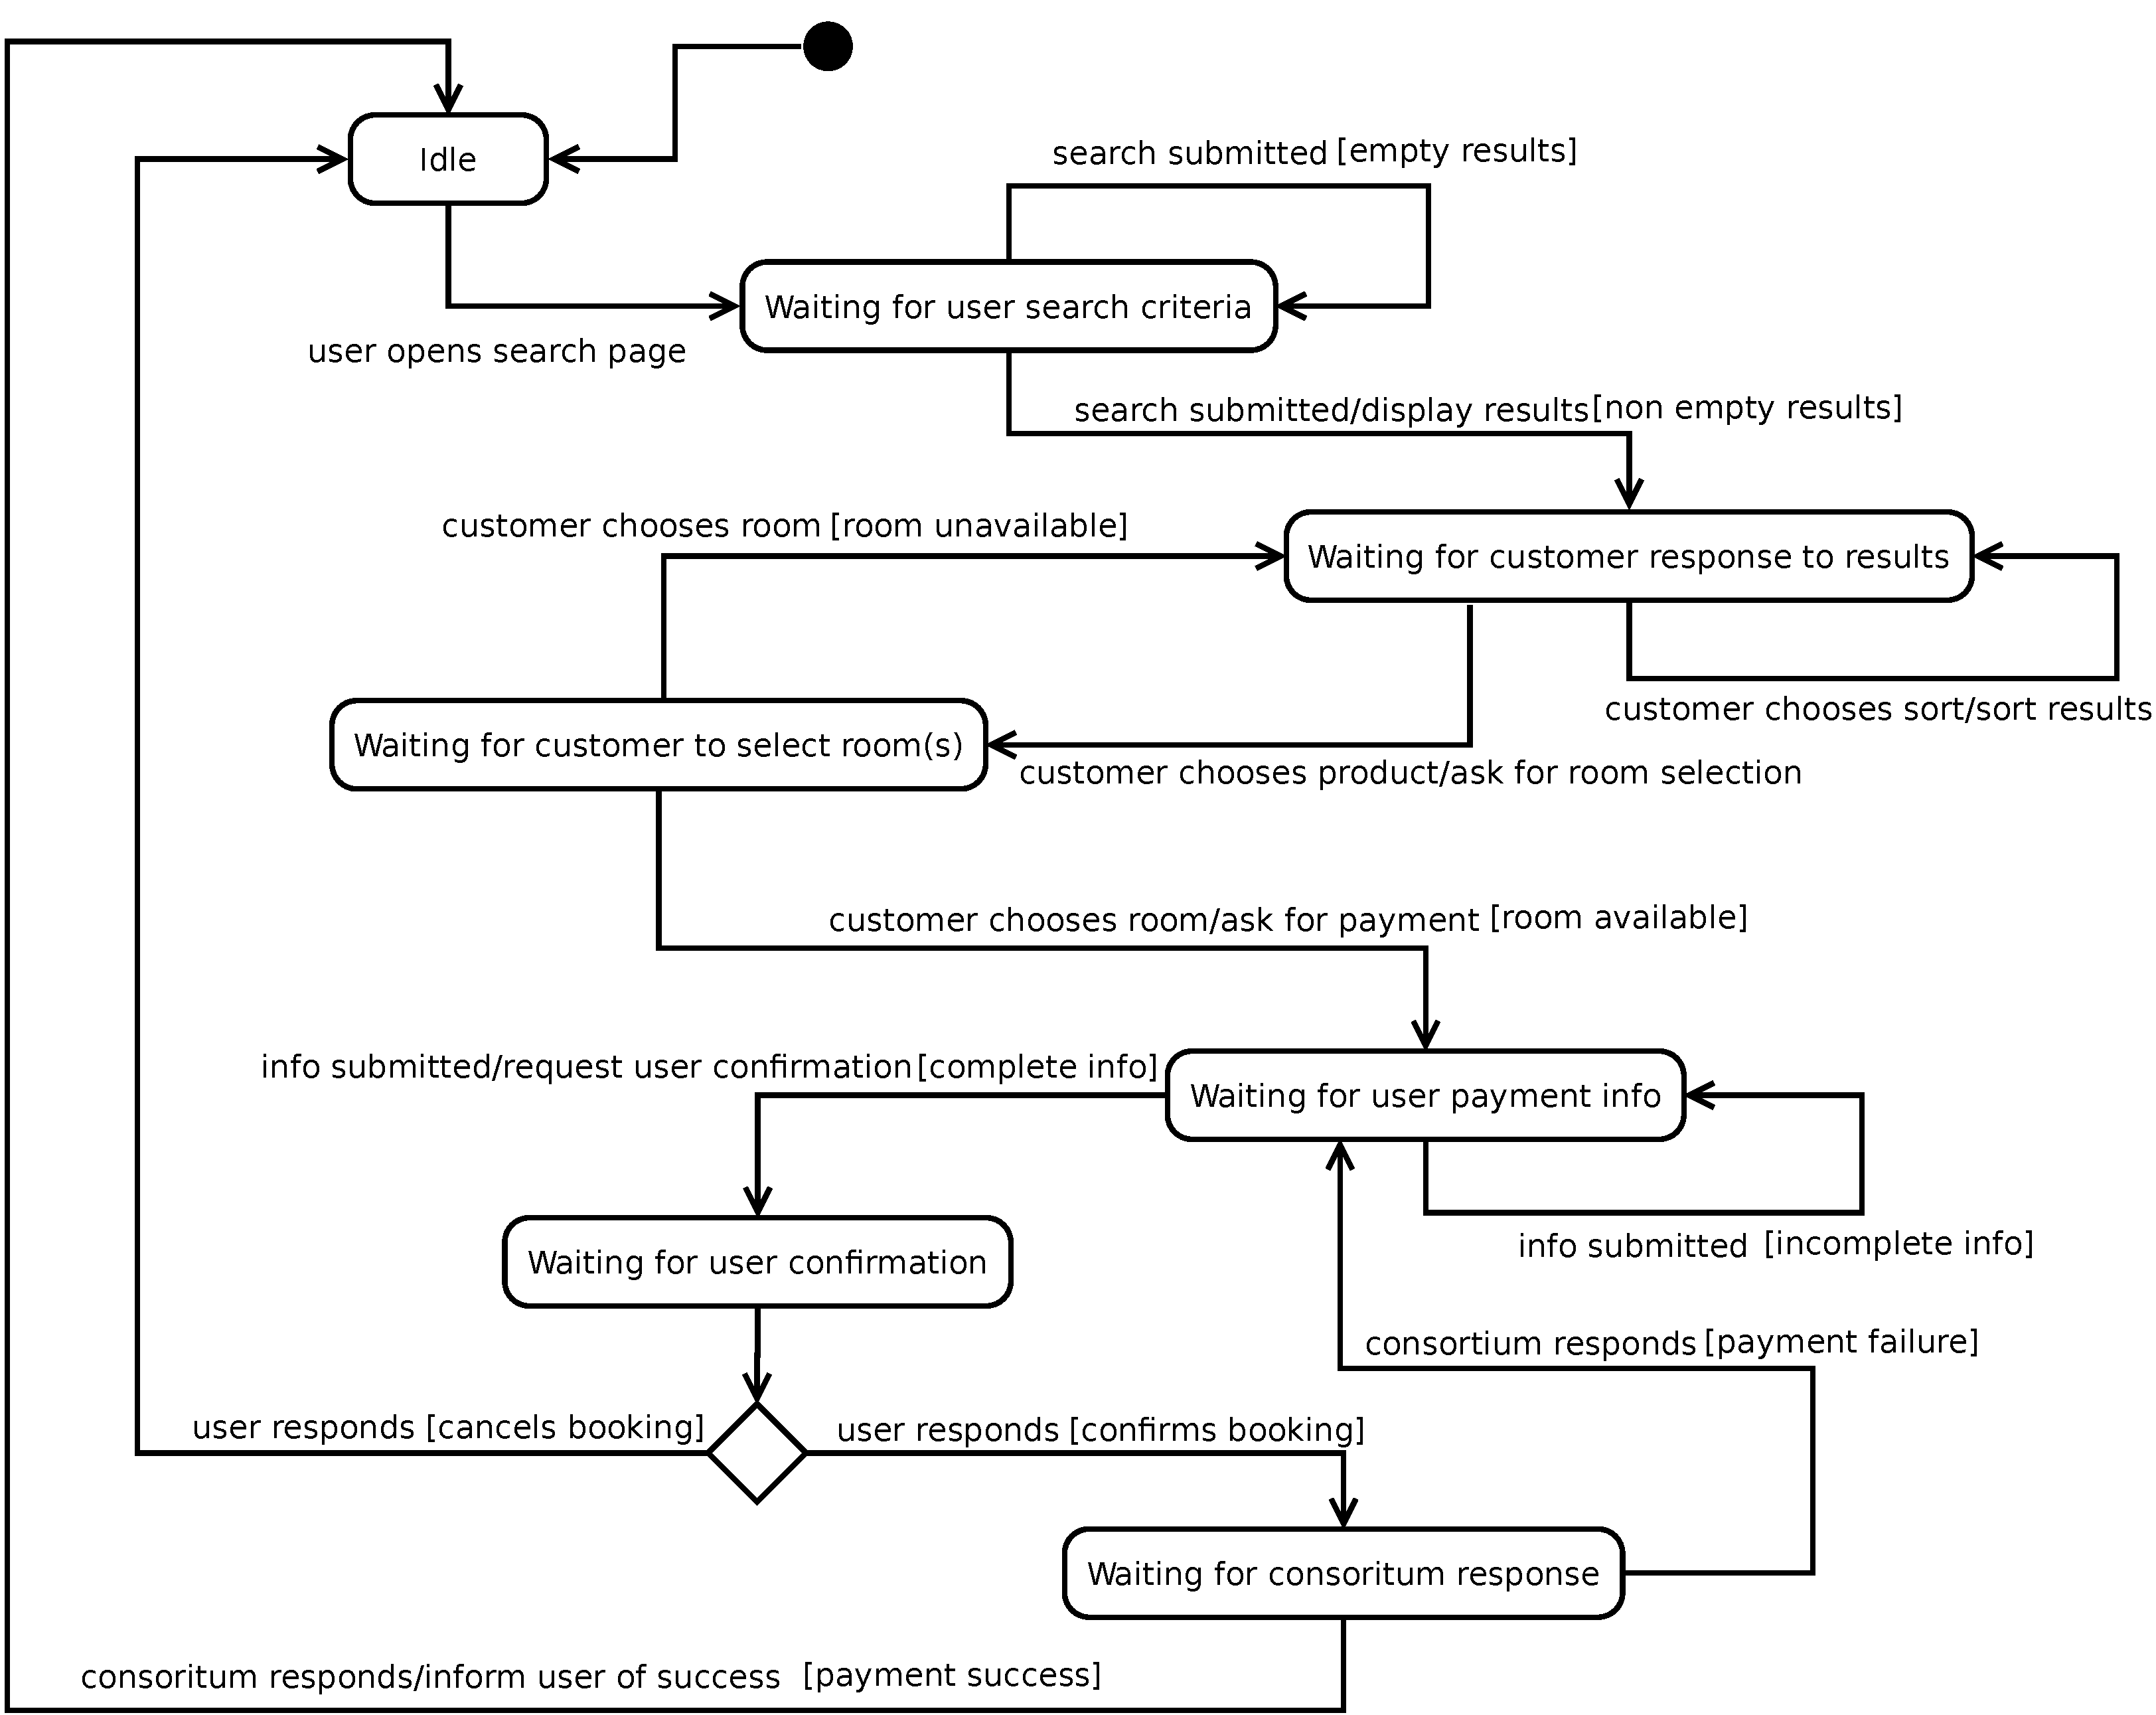
\includegraphics[width=1.1\textwidth]{../StateDiagram/StateDiagram.pdf}}%
	\caption{State diagram}
\end{figure}
\clearpage

\section{Component Diagram}
\begin{figure}[h!]
	\centering
	\makebox[\textwidth][c]{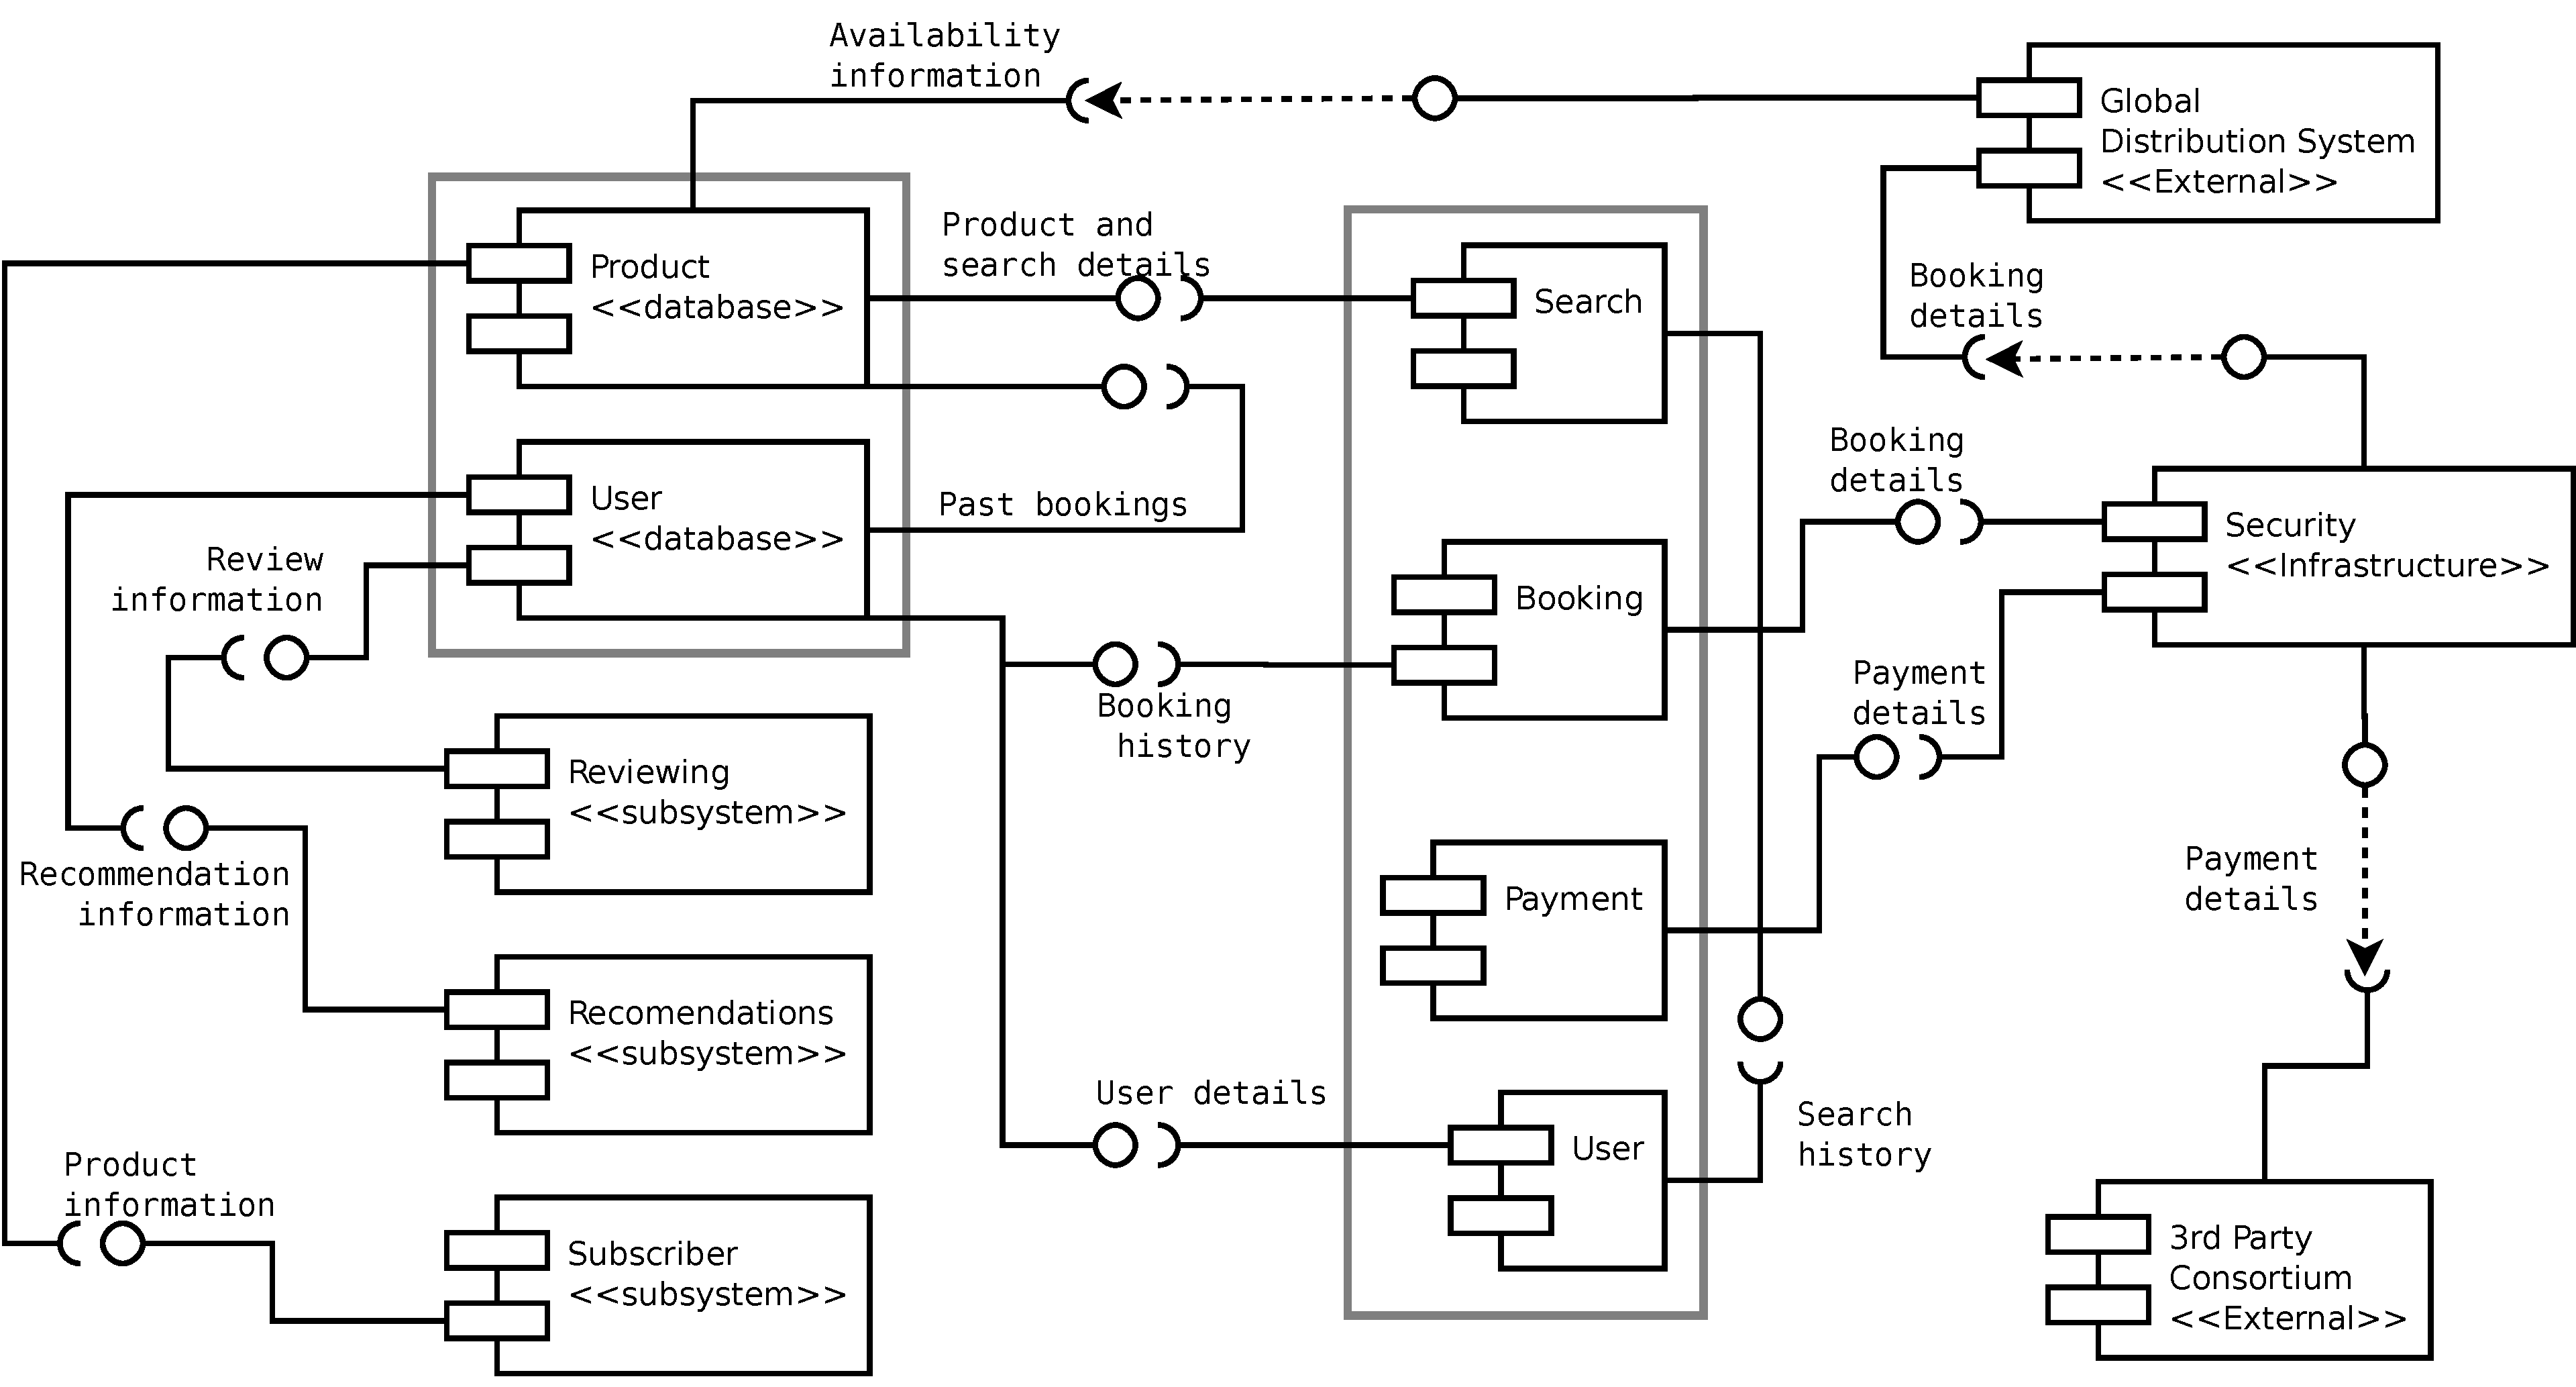
\includegraphics[angle=90,height=0.91\textheight]{../ComponentDiagram/ComponentDIagram.pdf}}%
	\caption{Component diagram}
\end{figure}
\clearpage

\section{Deployment Diagrams}

The first deployment diagram shows a possible implementation of a three tier
architecure. This incorporates the security aspects of the design separately in
the database and the business logic layers.

\begin{figure}[h!]
	\centering
	\makebox[\textwidth][c]{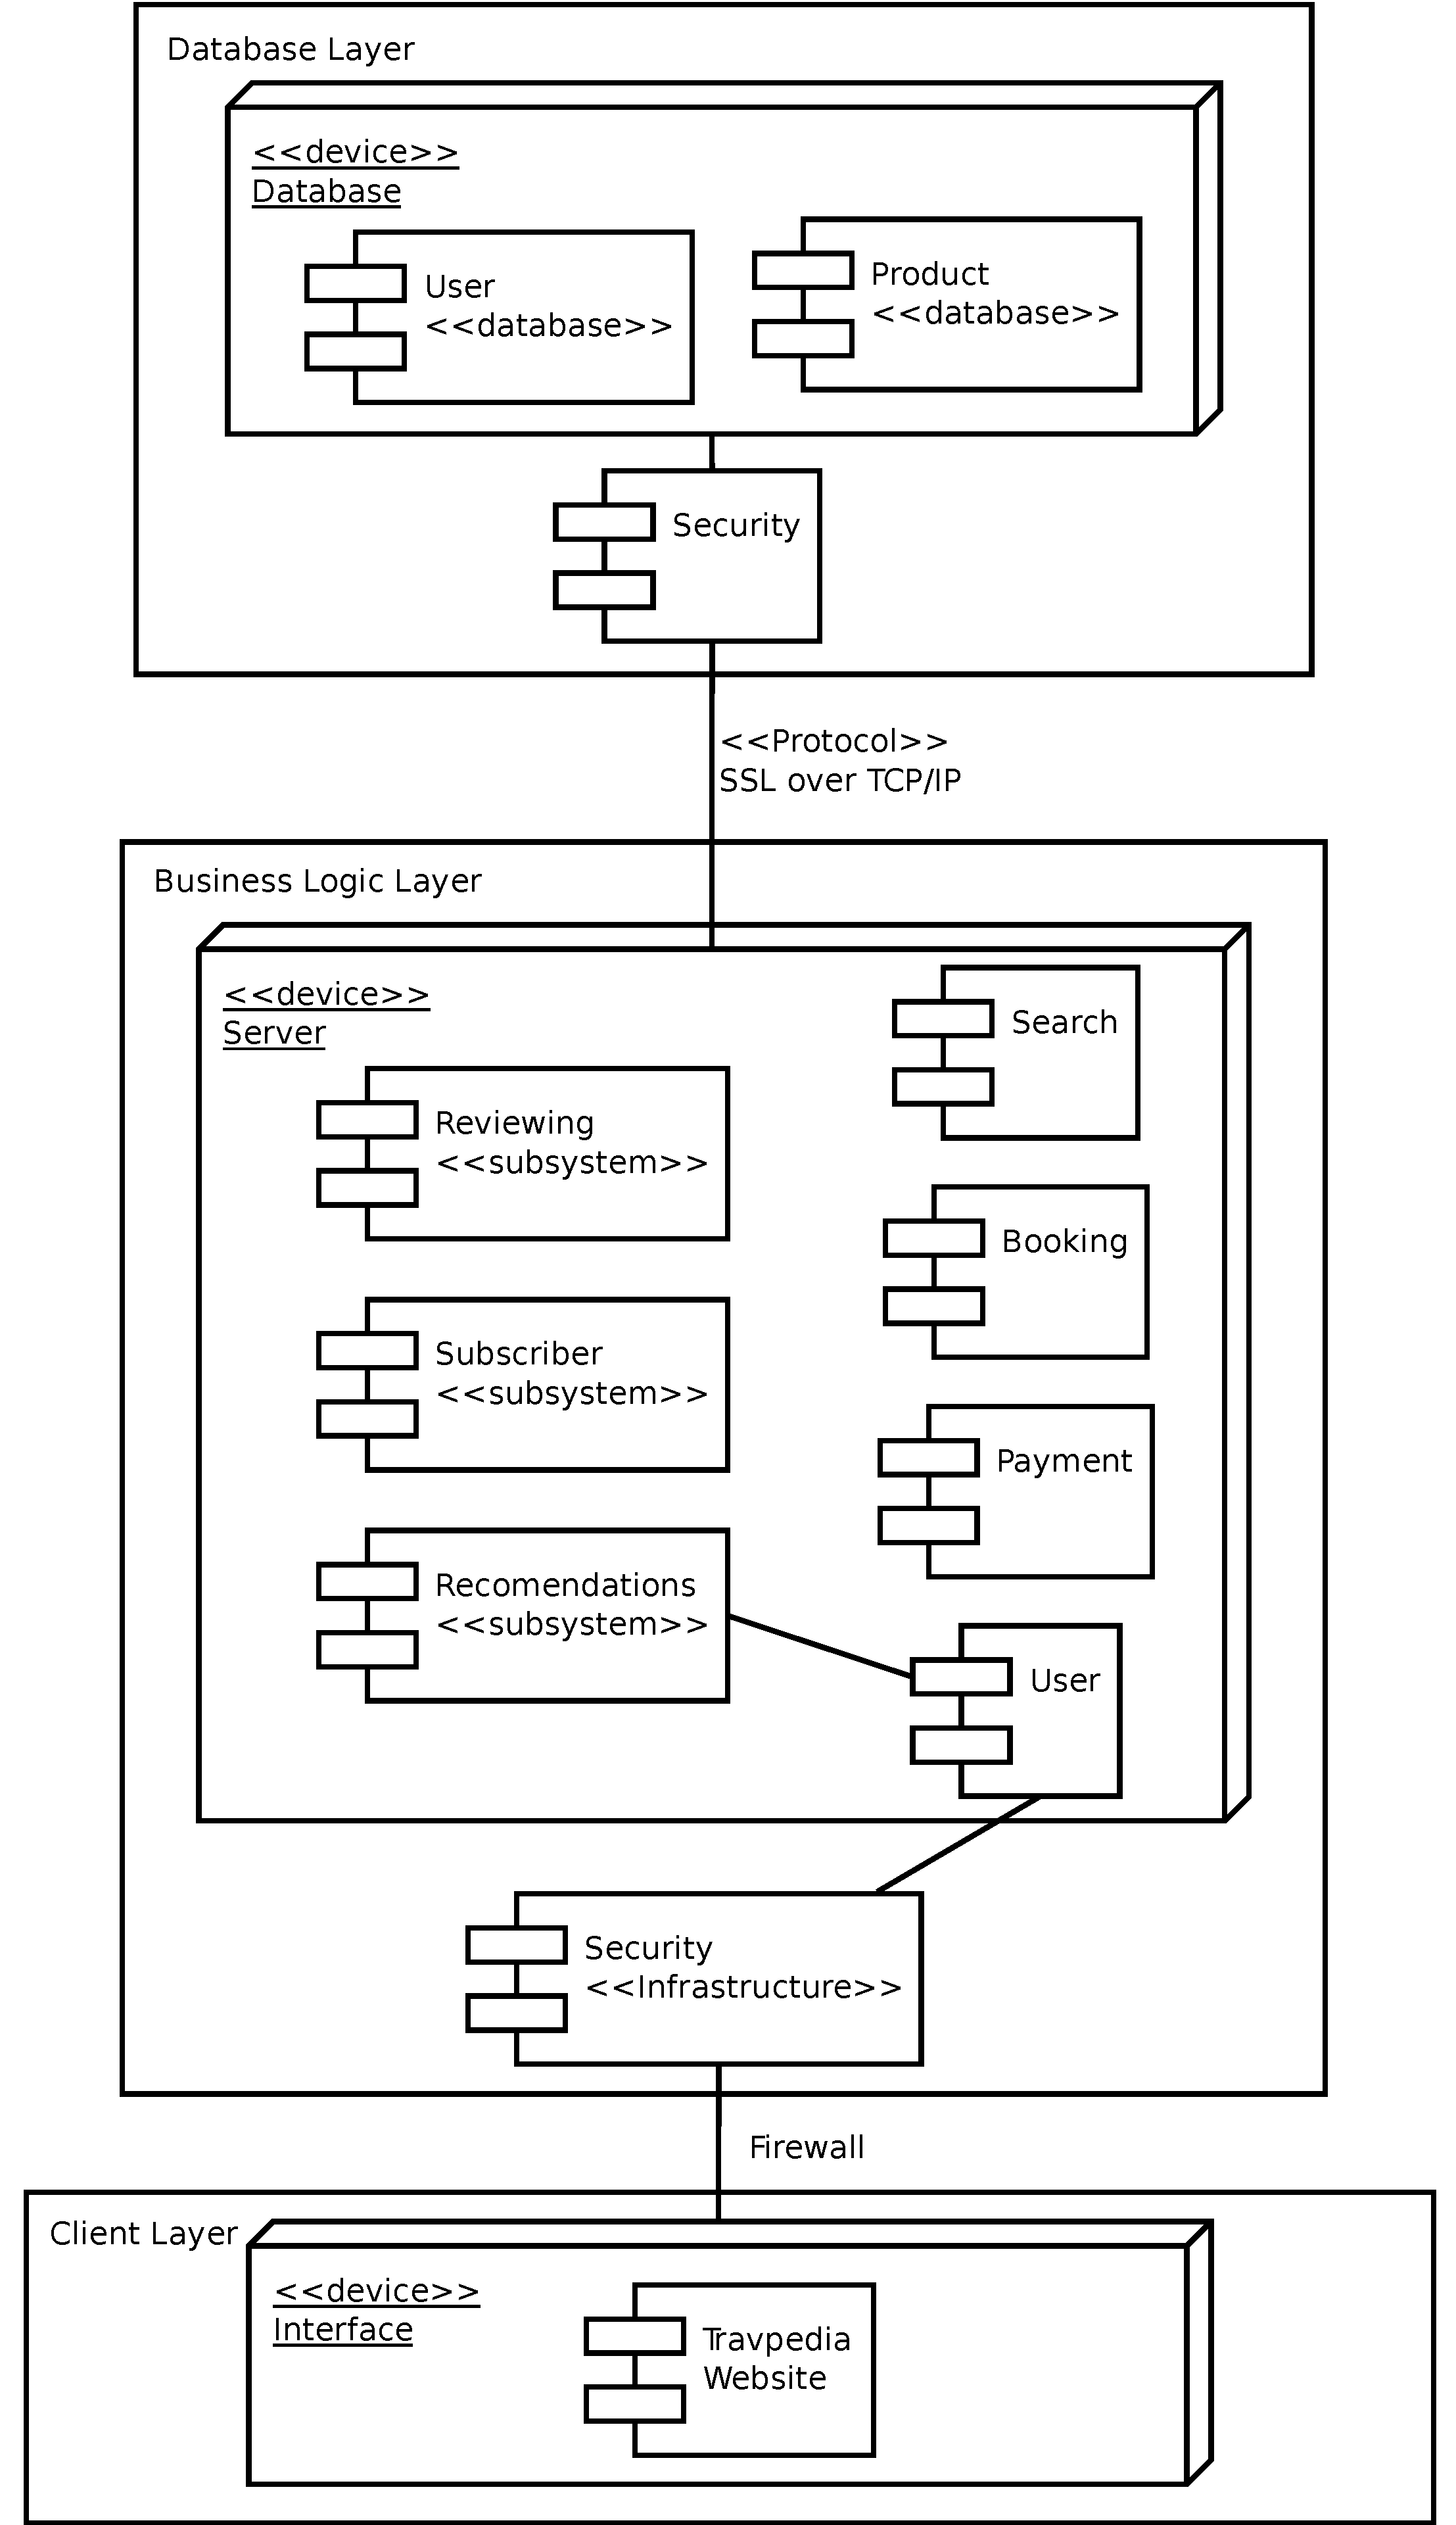
\includegraphics[height=0.85\textheight]{../DeploymentDiagram/deploymentDiag3tier.pdf}}%
	\caption{Three tier deployment diagram}
\end{figure}
\clearpage

The second deployment diagram shows a four tier architecure. This separates the
security aspects into a separate layer which means that the security can be
handled by a single system rather than being separated across different layers.

Were this system to be built, we would recommend the four tier architecture
shown here as this reduces overall complexity (since elements are not
duplicated) and so improves reliability as well as increasing security.

\begin{figure}[h!]
	\centering
	\makebox[\textwidth][c]{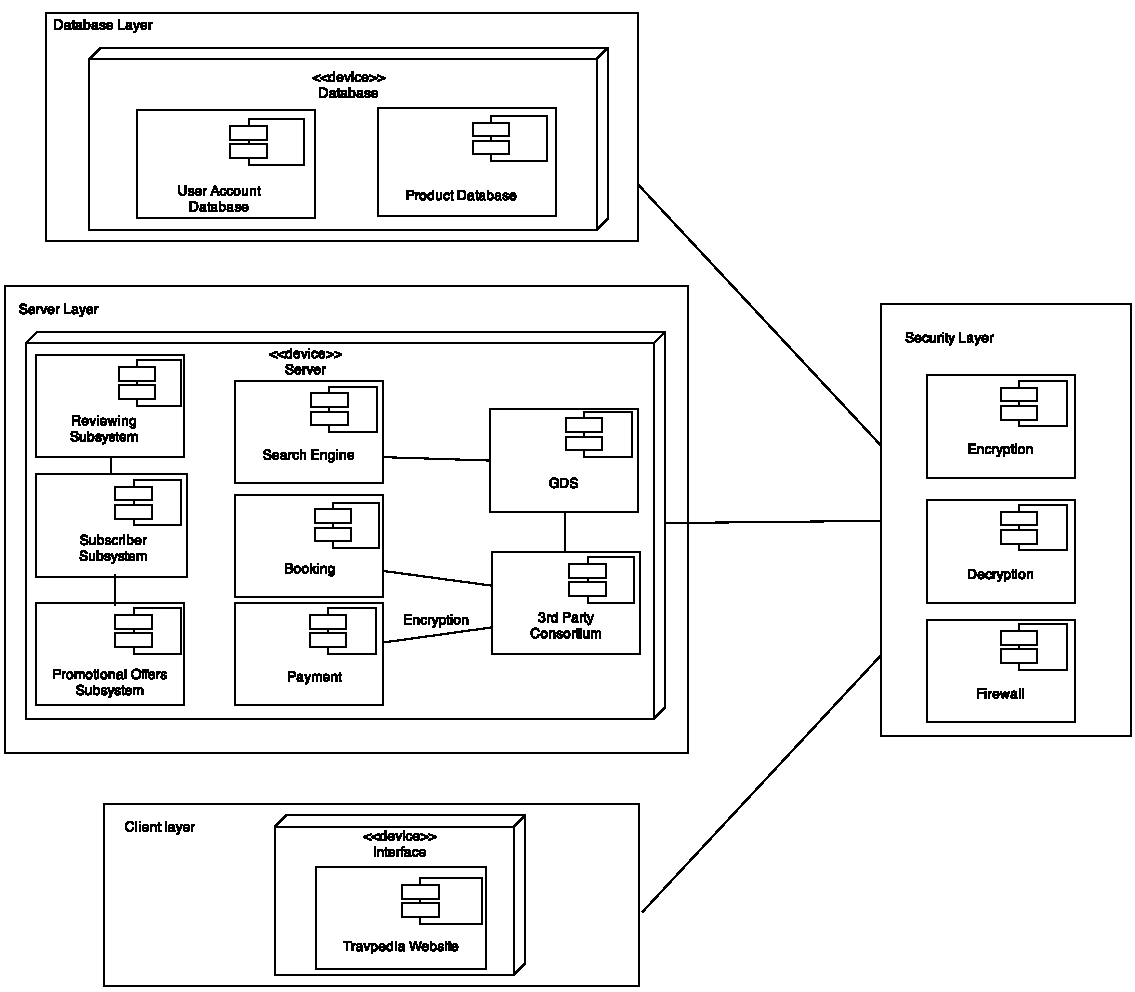
\includegraphics[angle=90,width=1.2\textwidth]{../DeploymentDiagram/deploymentDiag4tier.pdf}}%
	\caption{Four tier deployment diagram}
\end{figure}
\clearpage

\end{document}

% vim: autochdir
